\chapauthor{Никифоров С.А.\\Гойло А.А.\\Крощенко А.А.\\Захарьев В.А.\\Цянь Л.}
\chapter{Естественно-языковые интерфейсы ostis-систем}
\chapauthortoc{Никифоров С.~А.\\Гойло А.~А.\\Крощенко А.~А.\\Захарьев В.~А.\\Цянь Л.}
\label{chapter_nl_interfaces}

\begin{SCn}
	\begin{scnrelfromlist}{автор}
		\scnitem{Цянь Л.}
	\end{scnrelfromlist}
\end{SCn}

\bigskip

\abstract{
    В данной главе рассматривается подход к реализации естественно-языковых интерфейсов интеллектуальных компьютерных систем нового поколения, построенных по технологии OSTIS, а также предлагается модель контекста диалога.
    В данном подходе все этапы анализа, включая лексический, синтаксический и семантический анализ могут производиться непосредственно в базе знаний такой системы. Такой подход позволит эффективно решать такие задачи как управление глобальным и локальным контекстами диалога, а также разрешение языковых явлений таких как анафоры, омонимия и эллиптические фразы.

    \begin{textitemize}
        \item расписать сопоставление токенов с лексемами;
        \item перерисоват ькартинки, чать из них предназначалась для размещения в колонке;
        \item расписать синтаксический анализ, как находятся составляющие,
        \item пройтись по подсказкам от плагина, поправит форматирование,
        \item формализовать пр. о..
    \end{textitemize}
    Список вопросов:
    \begin{textitemize}
        \item что придумать с аналогичными картинками, как те, что были использованы в главе про языки - дублировать в одной книге плохо, но ссылаться чрез 100 страниц тоже.
    \end{textitemize}
}

\bigskip

\begin{SCn}
	\begin{scnrelfromlist}{подраздел}
		\scnitem{\ref{section_chinese_interfaces}~\nameref{section_chinese_interfaces}}
	\end{scnrelfromlist}

\bigskip

	\begin{scnrelfromlist}{библиографическая ссылка}
		\scnitem{\scncite{Wu2019}}
		\scnitem{\scncite{Liu2020}}
		\scnitem{\scncite{Abu2020}}
		\scnitem{\scncite{Xu2016}}
		\scnitem{\scncite{Liu2020}}
		\scnitem{\scncite{Tseng2014}}
		\scnitem{\scncite{Gatt2017}}
		\scnitem{\scncite{Androutsopoulos2013}}
		\scnitem{\scncite{Devlin2018}}
		\scnitem{\scncite{Brown2020}}		
		\scnitem{\scncite{Moryossef2019}}		
		\scnitem{\scncite{Gardent2017}}
		\scnitem{\scncite{Lehmann2015}}
		\scnitem{\scncite{Xu2017}}
		\scnitem{\scncite{Niu2011}}
		\scnitem{\scncite{Golenkov2014a}}
		\scnitem{\scncite{Hardzei2022}}	
		\scnitem{\scncite{Liu2006}}
		\scnitem{\scncite{Wang2006}}
		\scnitem{\scncite{Shunkevich2017}}
		\scnitem{\scncite{Qian2022}}
		\scnitem{\scncite{Davydenko2018}}
		\scnitem{\scncite{Shunkevich2018}}
		\scnitem{\scncite{Davydenko2017}}		
		\scnitem{\scncite{IMS}}
		\scnitem{\scncite{Li2022}}		
		\scnitem{\scncite{Trisedya2018}}
		\scnitem{\scncite{Kale2020}}
	\end{scnrelfromlist}
\end{SCn}

\bigskip

%Введение
В настоящее время существует большое количество различных интерфейсов компьютерных систем, что усложняет интероперабельность между такими системами и людьми в силу необходимости ознакомления с интерфейсом каждой новой системы, который зачастую может быть не интуитивно понятен.

Одной из основных особенностей интеллектуальных компьютерных систем нового поколения должен являться пользовательский интерфейс, способный обеспечить эффективное взаимодействие пользователя с системой в условиях его общей профессиональной неподготовленности.

Одной из наиболее естественных и удобных форм передачи информации между людьми является речь, что обуславливает все большее распространение естественно-языковых интерфейсов\scncite{GlobalMarket}. В настоящий момент времени уже ни у кого не вызывает сомнения, что данная форма взаимодействия человека и машины играет и будет играть значительную роль во взаимодействии с различными компьютерными системами.

Однако необходимо отметить, что большое многообразие языков (как естественных, так и искусственных) ведет к необходимости упрощения процесса создания таких интерфейсов для каждого отдельно взятого языка.

%Анализ
В основе большинства подходов к обработке и пониманию естественного языка лежит машинное обучение\scncite{NLP_as_a_service},\scncite{NLP_in_pharmacology}. Несомненно, для большинства широко распространенных языков модели для обработки естественного языка работают очень хорошо и совершенствуются с каждым днем, но несмотря на успехи в данной области, данный подход имеет ряд недостатков:
\begin{textitemize}
    \item проблемы при работе с различными областями, например, значения слов или предложений могут быть различными в зависимости от предметной области. Таким образом, модели для NLP могут хорошо работать для отдельной предметной области, но не подходить для широкого применения\scncite{NLPOverview};
    \item создание новой модели модели требует наличия большого объема данных, а качество таких данных напрямую влияет на качество получаемой модели, что ведет к большим затратам на ее обучение\scncite{strubell2019energy}\scncite{large_language_models};
    \item данные модели представляют собой "черный ящик"{}, т. к. данные модели не обладают средствами для обоснования своего вывода;
    \item каждая такая модель решает только свой узкий класс задач, отсутствует общий подход к обработке естественного языка.\scncite{NLPOverview}
\end{textitemize}

Данные недостатки используемых методов являются причиной части недостатков современных систем, реализующих естественно-языковой интерфейс, так, несмотря на то, что сейчас существует большое количество речевых ассистентов, создаваемых разными компаниями\scncite{site_url_alexa},\scncite{site_url_siri},\scncite{site_url_gassist},\scncite{site_url_cortana}, они обладают схожими недостатками, например, исключительно распределенной реализацией, в силу недостаточной для запуска ресурсоемких моделей производительности устройств конечных пользователей. Это в свою очередь ведет к проблемам с приватностью\scncite{PVA}.

Подмодуль понимания речи данных систем формирует конструкцию, отражающую смысл сообщения используя фреймовую модель. Упрощенный пример такой конструкции приведен на рисунке \textit{\nameref{fig:message_intents}}.

\begin{figure}[h]
    \centerline{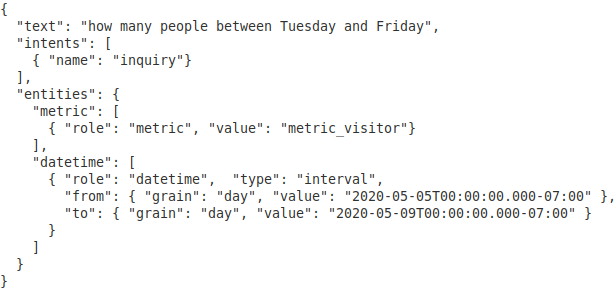
\includegraphics[width=\linewidth]{images/part4/chapter_nl_interfaces/message_intents.png}}
    \caption{Пример формализованного смысла сообщения}
    \label{fig:message_intents}
\end{figure}

При этом для представления результатов промежуточных этапов обработки используются иные форматы, модули которые их реализуют не имеют какой-либо единой основы и взаимодействуют посредством специализированных программных интерфейсов между ними, что приводит к несовместимости способов представления результатов на различных этапах обработки и конечного результата обработки текстов. Данная несовместимость в свою очередь ведет к существенным накладным расходам при разработке такой системы и в особенности при ее модификации.

В качестве решения проблемы совместимости предлагается использование подхода к обработке естественного языка на основе его формальной модели в виде набора онтологий, сформированных с использованием универсальных средств представления знаний, что будет способствовать интероперабельности как компонента по обработке естественного языка в целом с другими компонентами системы, так и между составляющими самого данного компонента.

Целью главы является формирование модели интерфейса, в основе которой лежит подход к обработке естественного языка на основе онтологий, содержащих формальное описание естественного языка.

\section{Предметная область и онтология естественно-языковых интерфейсов ostis-систем}

\textit{Естественно-языковой интерфейс} -- SILK-интерфейс (Speech – речь, Image – образ, Language – язык, Knowledge – знание), обмен информацией между компьютерной системой и пользователем в котором происходит за счёт диалога. Диалог ведётся на одном из естественных языков.

\begin{SCn}

    \scnheader{естественно-языковой интерфейс}
    \scnsuperset{речевой интерфейс}

\end{SCn}

\textit{Речевой интерфейс} -- SILK-интерфейс, обмен информацией в котором происходит за счёт диалога, в процессе которого компьютерная система и пользователь общаются с помощью речи. Данный вид интерфейса наиболее приближен к естественному общению между людьми.

В предлагаемом подходе можно выделить следующие этапы обработки естественного языка:
\begin{textitemize}
    \item лексический анализ;
    \item синтаксический анализ;
    \item понимание сообщения.
\end{textitemize}

В свою очередь, лексический анализ в включает в себя декомпозицию текста на токены и их сопоставление с лексемами.

Понимание сообщения сводится к генерации вариантов значения сообщения и выбору из них корректного на основании контекста, а также погружение его в данный контекст.

Ниже приведена структура решателя задач естественно-языкового интерфейса.

\begin{SCn}

    \scnheader{Решатель задач естественно-языкового интерфейса}
    \begin{scnrelfromset}{декомпозиция абстрактного sc-агента}
        \scnitem{Абстрактный sc-агент лексического анализа}
        \begin{scnindent}
            \begin{scnrelfromset}{декомпозиция абстрактного sc-агента}
                \scnitem{Абстрактный sc-агент декомпозиции текста на токены}
                \scnitem{Абстрактный sc-агент сопоставления токенов с лексемами}
            \end{scnrelfromset}
        \end{scnindent}
        \scnitem{Абстрактный sc-агент синтаксического анализа}
        \scnitem{Абстрактный sc-агент понимания сообщения}
    \end{scnrelfromset}

\end{SCn}

В свою очередь, \textit{Абстрактный sc-агент понимания сообщения} декомпозируется на:

\begin{SCn}

    \scnheader{Агент понимания сообщения}
    \begin{scnrelfromset}{декомпозиция абстрактного sc-агента}
        \scnitem{Абстрактный sc-агент генерации вариантов значения сообщения}
        \scnitem{Абстрактный sc-агент выбора и обновления контекста}
        \begin{scnindent}
            \begin{scnrelfromset}{декомпозиция абстрактного sc-агента}
                \scnitem{Абстрактный sc-агент разрешения контекста}
                \scnitem{Абстрактный sc-агент выбора смысла сообщения на основе контекста}
                \scnitem{Абстрактный sc-агент погружения сообщения в контекст}
            \end{scnrelfromset}
        \end{scnindent}
    \end{scnrelfromset}

\end{SCn}

Для каждого агента в базе знаний должна находиться спецификация, пример фрагмента такой спецификации приведен на рисунке \textit{\nameref{fig:agent_spec}}.

\begin{figure}[h]
    \centering
    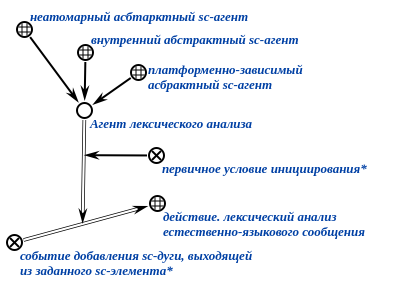
\includegraphics[width=0.4\textwidth]{images/part4/chapter_nl_interfaces/agent_spec.png}
    \caption{Пример спецификации агента.}
    \label{fig:agent_spec}
\end{figure}

\section{Предметная область и онтология лексического анализа естественно-языковых сообщений, входящих в ostis-систему}

\begin{SCn}

    \scnheader{действие. лексический анализ естественно-языкового сообщения}
    \begin{scnrelfromset}{обобщенная декомпозиция}
        \scnitem{действие. декомпозиция текста на токены}
        \scnitem{действие. сопоставление токенов с лексемами}
    \end{scnrelfromset}

\end{SCn}

С точки зрения ostis-системы, любой естественно-языковой текст является \textit{файлом} (т.е. SC-узлом с содержимым).

Этап лексического анализа представляет собой декомпозицию текста на последовательность токенов и сопоставление лексем с получившимися при данной декомпозиции токенами. Следует отметить, что данные токены при необходимости могут сопоставляться не с лексемами, а с их подмножествами, входящими в ее морфологическую парадигму, соответствующими определенным грамматическим категориям: падежу, числу, роду и т.д.

Результат лексического анализа представлен на рисунке \textit{\nameref{fig:lexical_result}}.

\begin{figure}[h]
    \centering
    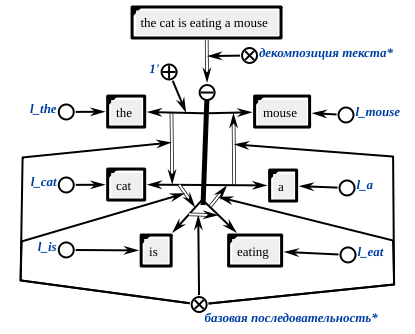
\includegraphics[width=0.4\textwidth]{images/part4/chapter_nl_interfaces/lexical.png}
    \caption{Пример результата лексического анализа.}
    \label{fig:lexical_result}
\end{figure}

Для осуществления лексического анализа, в базе знаний системы также должен присутствовать словарь, содержащий лексемы и их различные формы.

Под лексемой понимается единица словарного состава языка, которая представляет собой множество всех форм некоторого слова.
Пример спецификации лексемы в базе знаний приведен на рисунке \textit{\nameref{fig:lexeme_example}}.

\begin{figure}[h]
    \centering
    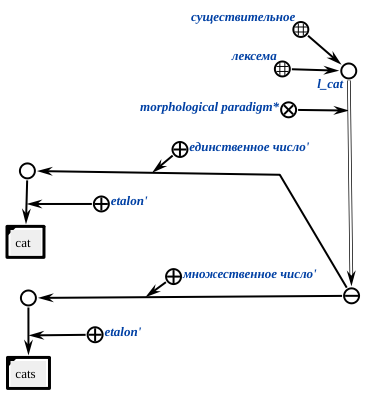
\includegraphics[width=0.4\textwidth]{images/part4/chapter_nl_interfaces/lexeme_example.png}
    \caption{Пример спецификации лексемы в базе знаний.}
    \label{fig:lexeme_example}
\end{figure}

\section{Предметная область и онтология синтаксического анализа естественно-языковых сообщений, входящих в ostis-систему}

Агент синтаксического анализа выполняет переход от размеченного на лексемы текста к его синтаксической структуре.
При этом из-за невозможности разрешения структурной неоднозначности на этапе синтаксического анализа, его результатом в общем случае будет являться множество потенциальных синтаксических структур.

Пример одной синтаксической структуры представлен на рисунке \textit{\nameref{fig:syntactic_result}}.

\begin{figure*}[h]
    \centering
    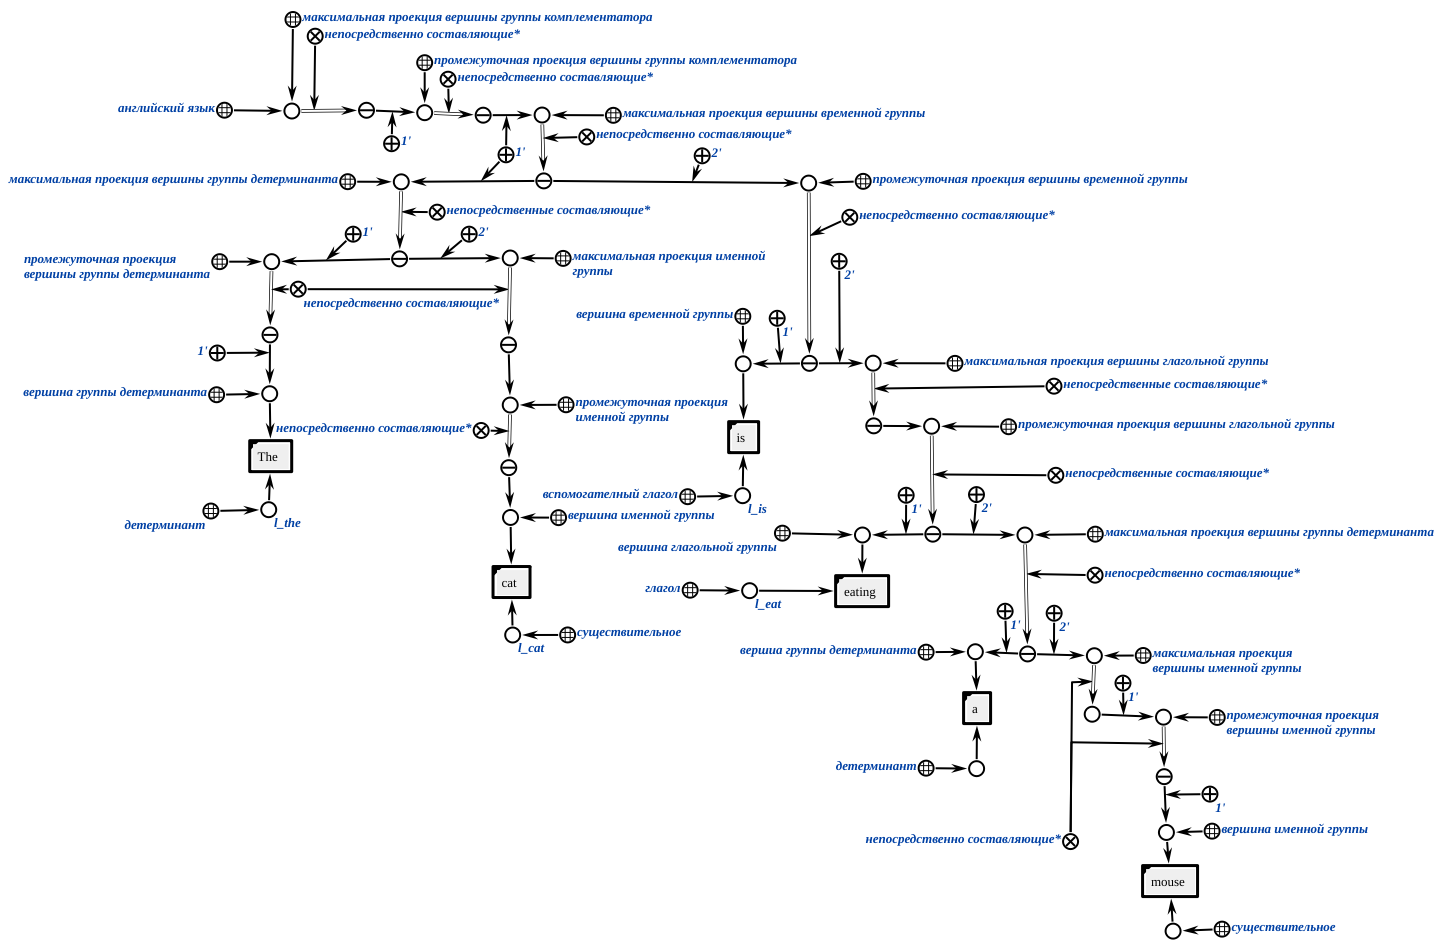
\includegraphics[width=\textwidth]{images/part4/chapter_nl_interfaces/syntactic.png}
    \caption{Пример синтаксической структуры.}
    \label{fig:syntactic_result}
\end{figure*}


\section{Предметная область и онтология понимания естественно-языковых сообщений, входящих в ostis-систему}

\begin{SCn}

    \scnheader{действие. понимание естественно-языкового сообщения}
    \begin{scnrelfromset}{обобщенная декомпозиция}
        \scnitem{действие. генерация вариантов значения сообщения}
        \scnitem{действие. выбор и обновление контекста}
        \begin{scnindent}
            \begin{scnrelfromset}{обобщенная декомпозиция}
                \scnitem{действие. разрешение контекста}
                \scnitem{действие. выбор смысла сообщения на основе контекста}
                \scnitem{действие. погружение сообщения в контекст}
            \end{scnrelfromset}
        \end{scnindent}
    \end{scnrelfromset}

\end{SCn}

\textit{Действие. генерация вариантов значения сообщения} -- действие, в ходе которого осуществляется формирование строгой дизъюнкции потенциально эквивалентных структур.

\textit{Потенциально эквивалентная структура*} -- бинарное ориентированное отношение, связывающее структуру и множество структур, которые потенциально могут быть эквивалентны ей, однако для достоверного определения факта требуются дополнительные действия.

При этом, переход от результата синтаксического анализа к потенциально эквивалентным сообщению структурам осуществляется по правилам, содержащихся в предметной области денотационной семантики. Пример одного из правил представлен на рисунке \textit{\nameref{fig:transition_to_semanic_rule}}.

\begin{figure*}[h]
    \centering
    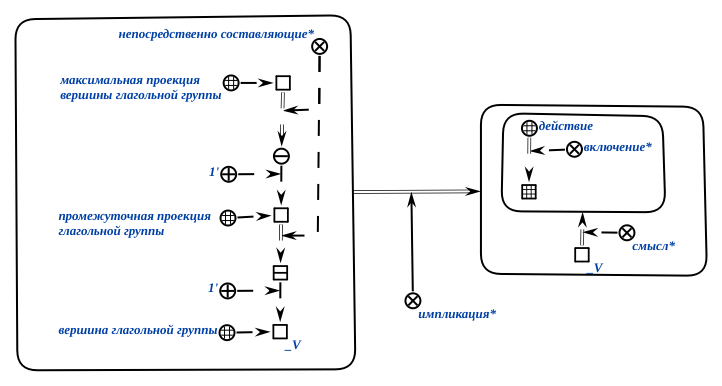
\includegraphics[width=0.7\textwidth]{images/part4/chapter_nl_interfaces/d_sem_3.png}
    \caption{Пример правила перехода от синтаксической структуры к семантике.}
    \label{fig:transition_to_semanic_rule}
\end{figure*}

В результате данного действия в базе знаний формируется структура, описывающая возможные варианты смысла сообщения, пример такой структуры в терминах грамматики составляющих\scncite{X_bar_syntax} приведен на \textit{\nameref{fig:messsage_meaning_variants}}. Наличие нескольких таких структур объясняется тем, что в общем случае на этапе синтаксического анализа выполняется генерация нескольких вариантов синтаксической структуры. Выбор корректного значения сообщения будет осуществлен в ходе выполнения последующих действий.

\begin{figure}[h]
    \centering
    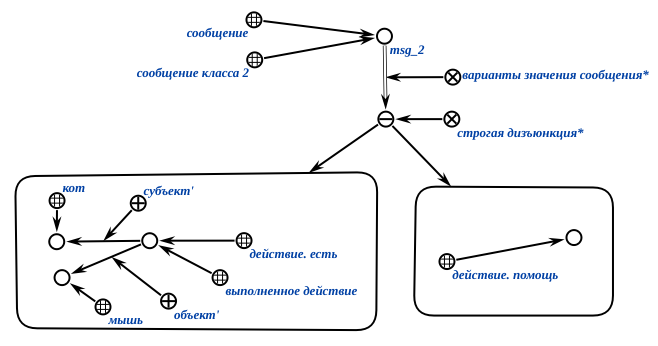
\includegraphics[width=0.45\textwidth]{images/part4/chapter_nl_interfaces/messsage_meaning_variants.png}
    \caption{Пример конструкции, описывающей потенциальные смыслы сообщения.}
    \label{fig:messsage_meaning_variants}
\end{figure}

Следует отметить, что при необходимости смысл сообщения может быть сгенерирован не только на основании его синтаксической структуры в терминах грамматики составляющих, но и других знаний о данном сообщении, например выделенных из текста данного сообщения троек вида субъект-отношение-объект, результата его классификации и т. п.

Дальнейшие этапы процесса понимания сообщения выполняются на основе контекста.

\textit{Контекст} - sc-структура, содержащая знания, которыми оперирует система в ходе одного или нескольких диалогов.
В общем случае, данные знания включают в себя как предварительно занесенные в БЗ, так и полученные в ходе работы с сенсоров и/или диалога.

\begin{SCn}

    \scnheader{контекст диалога}
    \scnsubset{контекст}
    \scnrelfrom{subdividing}{\scnkeyword{Типология контекстов диалога по глобальности\scnsupergroupsign}}
    \begin{scnindent}
        \begin{scneqtoset}
            \scnitem{тематический контекст}
            \scnitem{пользовательский контекст}
            \scnitem{глобальный контекст}
        \end{scneqtoset}
    \end{scnindent}

\end{SCn}

\textit{Тематический контекст} -- контекст диалога, содержащий специфические для темы сведения (сведения, полученные во время ведения диалога, на определенную тематику, например, при диалоге об определенном наборе сущностей).

\textit{Множество тематических контекстов диалога*} -- бинарное ориентированное отношение, диалог с ориентированным множеством его тематических контекстов.

\textit{Пользовательский контекст} -- контекст диалога, содержащие специфические для пользователя сведения, которые могут быть использованы в диалоге с ним на любую тематику. В общем случае пользовательский контекст имеет пересечение с согласованной частью БЗ (предварительно занесенная в БЗ достоверная информация о пользователе, прошедшая необходимую модерацию), но не включается в нее целиком (часть, полученная в ходе диалога в которой мы не уверены).
Пример соотнесения различных типов контекстов с согласованной частью базы знаний приведен на рисунке \textit{\nameref{fig:context_in_KB}}.

\textit{Глобальный контекст} -- контекст диалога, содержащий сведения, которые могут быть необходимы при ведении диалога с любым пользователем. Глобальный контекст -- подмножество согласованной части БЗ, содержащее те сведения, что допустимо использовать в диалоге. Например, в диалоге с определенным пользователем не нужно использовать:
\begin{itemize}
    \item находящуюся в базе знаний служебную информацию, необходимую для работы системы, но не предназначенную для использования в диалоге;
    \item части пользовательских контекстов иных пользователей.
\end{itemize}

\begin{figure}[h]
    \centering
    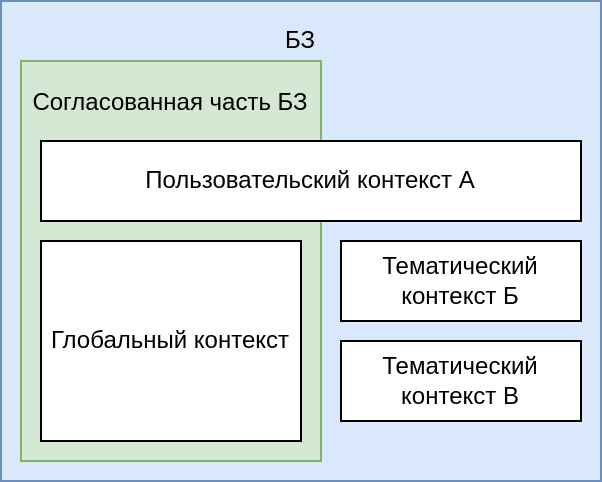
\includegraphics[width=0.4\textwidth]{images/part4/chapter_nl_interfaces/context_in_KB.png}
    \caption{Соотношение контекстов с согласованной частью баз знаний.}
    \label{fig:context_in_KB}
\end{figure}

\begin{SCn}

    \scnheader{контекст диалога}
    \scnrelfrom{subdividing}{\scnkeyword{Типология контекство по сроку достоверности знаний\scnsupergroupsign}}
    \begin{scnindent}
        \begin{scneqtoset}
            \scnitem{неизменяемый в ходе работы системы контекст диалога}
            \scnitem{изменяемый в ходе работы системы контекст диалога}
        \end{scneqtoset}
    \end{scnindent}

\end{SCn}

\textit{Неизменяемый в ходе работы системы контекст диалога} содержит в себе знания, необходимые для обеспечения выполнения системой своих функций,  которые были заложены в нее априорно ее разработчиками и/или администраторами и не изменяются в ходе ее функционирования на постоянной основе.

\textit{Изменяемый в ходе работы системы контекст диалога} содержит в себе знания, необходимые для обеспечения выполнения системой своих функций,  которые были ей получены в ходе ее работы и/или достоверность которых скоротечна.

\begin{SCn}


    \scnheader{изменяемый в ходе работы системы контекст диалога}
    \scnrelfrom{subdividing}{\scnkeyword{Типология изменяемых в ходе работы системы контекстов по источнику знаний\scnsupergroupsign}}
    \begin{scnindent}
        \begin{scneqtoset}
            \scnitem{контекст диалога, содержащий знания из внешних источников}
            \scnitem{контекст диалога, содержащий знания, полученные в ходе диалога}
        \end{scneqtoset}
    \end{scnindent}
    \scnrelfrom{subdividing}{\scnkeyword{Типология изменяемых контекстов по степени их достоверности\scnsupergroupsign}}
    \begin{scnindent}
        \begin{scneqtoset}
            \scnitem{достоверный контекст диалога}
            \scnitem{недостоверный контекст диалога}
        \end{scneqtoset}
    \end{scnindent}

\end{SCn}

Подмножество контекста может включаться в согласованную часть БЗ, например, если речь идет о каких-то предварительно занесенных в БЗ биографических сведениях -- дате рождения и т. п.

В каждый момент времени с пользователем связан 1 пользовательский диалоговый контекст (содержащий, по крайней мере известные заранее факты о нем: имя, возраст и т. п.) и несколько тематических.
Пример спецификации контекстов представлен на рисунке \textit{\nameref{fig:user_context}}.

\begin{figure}[h]
    \centering
    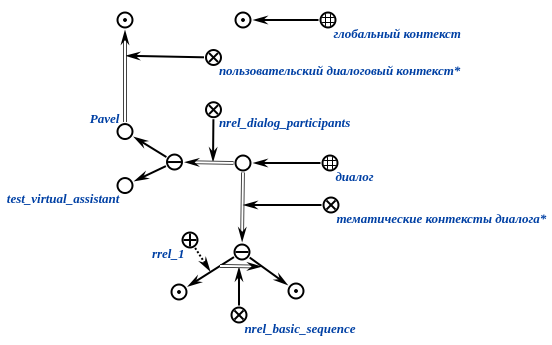
\includegraphics[width=0.5\textwidth]{images/part4/chapter_nl_interfaces/user_context.png}
    \caption{Пример спецификации контекстов.}
    \label{fig:user_context}
\end{figure}

Так, \textbf{действие. разрешение контекста} сводится к сопоставлению каждому варианту его значения соответствующего контекста.
Выбор производится на основании значения функции $F_{CTD}(T, C)$, где T - вариант трансляции, C - тематический контекст.
Подходящим контекстом для варианта трансляции считается тот, для которого значение этой функции максимально.
В случае, если подходящий контекст не найден, генерируется новый.
Пример результата данного действия представлен на рисунке \textit{\nameref{fig:relevant_contexts}}.

\begin{figure}[h]
    \centering
    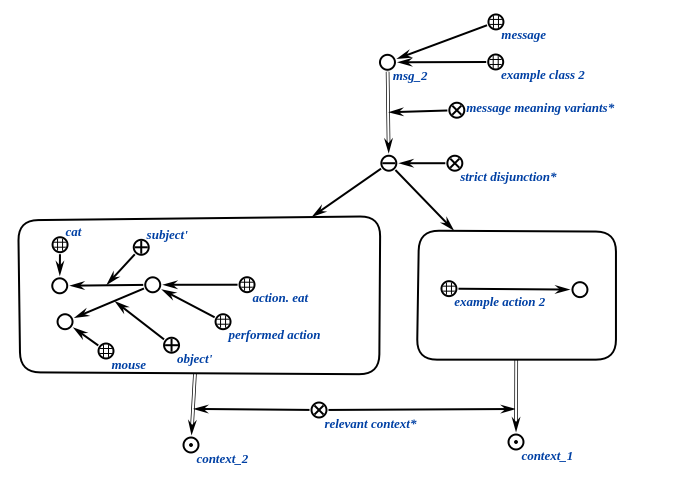
\includegraphics[width=0.45\textwidth]{images/part4/chapter_nl_interfaces/relevant_contexts.png}
    \caption{Пример сообщения, всем вариантам значения которого сопоставлен контекст.}
    \label{fig:relevant_contexts}
\end{figure}

\textbf{Действие. выбор смысла сообщения} представляет собой выбор из множества вариантов трансляции и соответствующих им контекстов одной пары и обозначение ее как эквивалентной сообщению конструкции. В простейшем случае, на данном этапе допустимо выполнить выбор в соответствии с рассчитанными на предыдущем этапе для пар потенциально эквивалентных структур и соответствующих им контекстов значениями функции $F_{CTD}(T, C)$ и выбрать пару, для которой оно максимально, однако при необходимости также возможно введение и отдельной функции.
Пример результата данного действия представлен на рисунке \textit{\nameref{fig:message_equivalent_structure}}.

\begin{figure}[h]
    \centering
    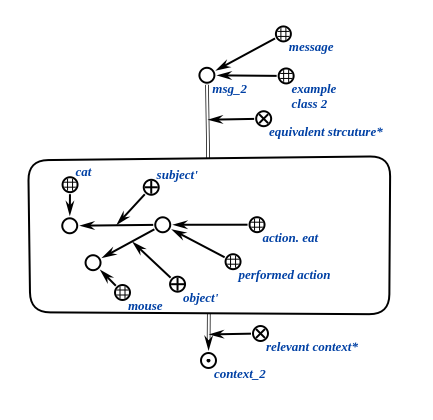
\includegraphics[width=0.35\textwidth]{images/part4/chapter_nl_interfaces/message_equivalent_structure.png}
    \caption{Пример конструкции, описывающей эквивалентную сообщению структуру.}
    \label{fig:message_equivalent_structure}
\end{figure}

\textbf{Действие. погружение сообщения в контекст} представляет собой погружение полученного смысла сообщения в контекст.
Кроме выбранного смысла сообщения, в контекст может добавляться и иная необходимая для обработки сообщения информация.
Кроме того, на данном этапе на основе хранящихся в контексте сведений также должно выполняться разрешение местоимений.
Примеры контекста до погружения в него сообщения и после погружения представлены на рисунках \textit{\nameref{fig:context_before_update}} и \textit{\nameref{fig:updated_context}}.

\begin{figure}[h]
    \centering
    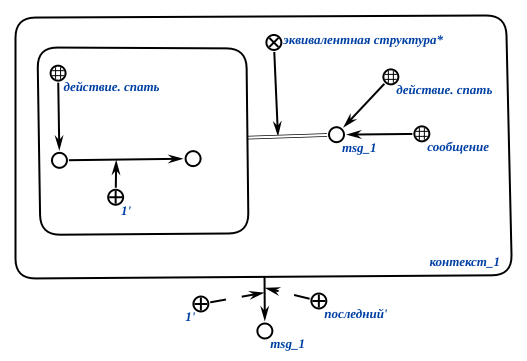
\includegraphics[width=0.4\textwidth]{images/part4/chapter_nl_interfaces/context_1.png}
    \caption{Пример контекста до погружения сообщения.}
    \label{fig:context_before_update}
\end{figure}

\begin{figure*}[h]
    \centering
    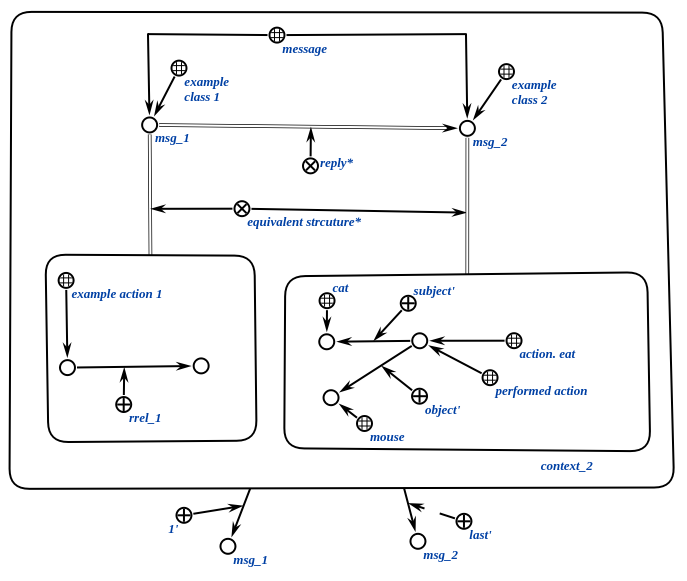
\includegraphics[width=0.7\textwidth]{images/part4/chapter_nl_interfaces/context_2.png}
    \caption{Пример контекста после погружения сообщения.}
    \label{fig:updated_context}
\end{figure*}

Таким образом, актуальная информация собирается в тематический контекст, объединив который с контекстом пользователя и глобальным контекстом можно получить общий контекст, на основании которого должны осуществляться требуемые действия системы, включая генерацию ответа системы.

%Под вопросом
\section{Предметная область и онтология синтеза естественно-языковых сообщений ostis-системы}
\section{Модели, методы и средства адаптации пользовательских интерфейсов к носителям китайского языка}
\label{section_chinese_interfaces}
Данный раздел посвящен рассмотрению разработки естественно-языковых интерфейсов интеллектуальных систем, ориентированных на решение задач преобразования текстов естественного языка в фрагменты базы знаний, и задач генерации текстов естественного языка из фрагментов базы знаний. Предложена семантическая модель естественно-языковых интерфейсов, которая включает в себя модель базы знаний лингвистики, а также модель решателей задач для решения данных двух задач в естественно-языковых интерфейсах, что позволяет проводить объединение лингвистических знаний на различных уровнях по обработке естественного языка в единую базу знаний, а также глубокую интеграцию различных моделей решения задач для обработки естественного языка. Описание принципов разработки китайско-языкового интерфейса осуществляется на основе предложенной единой модели естественно-языковых интерфейсов.

В настоящее время интерфейсы на основе распознавания текстов естественного языка, являются наиболее распространенными компонентами любых поисковых систем (например, Google, Yandex, Baidu и другие) или вопросно-ответных систем на основе базы знаний (см. \scncite{Wu2019}). В отличие от речевых интерфейсов, данные интерфейсы, как правило, ориентированы на обработку текстов естественного языка. В обычных современных поисковых системах вопросно-ответные системы начали разрабатываться как их подсистемы, ориентированные на обработку вопросительных предложений (или декларативных предложений).

Модульная схема (рисунок \textit{\nameref{fig:schema-natural-interface}})современных вопросно-ответных систем, основанных на знаниях описывает общий автоматизированный процесс информационного взаимодействия между текстами естественного языка (особенно вопросительными предложениями), предоставляемыми человеческими пользователями и базами знаний интеллектуальных систем.

\begin{figure}[H]
	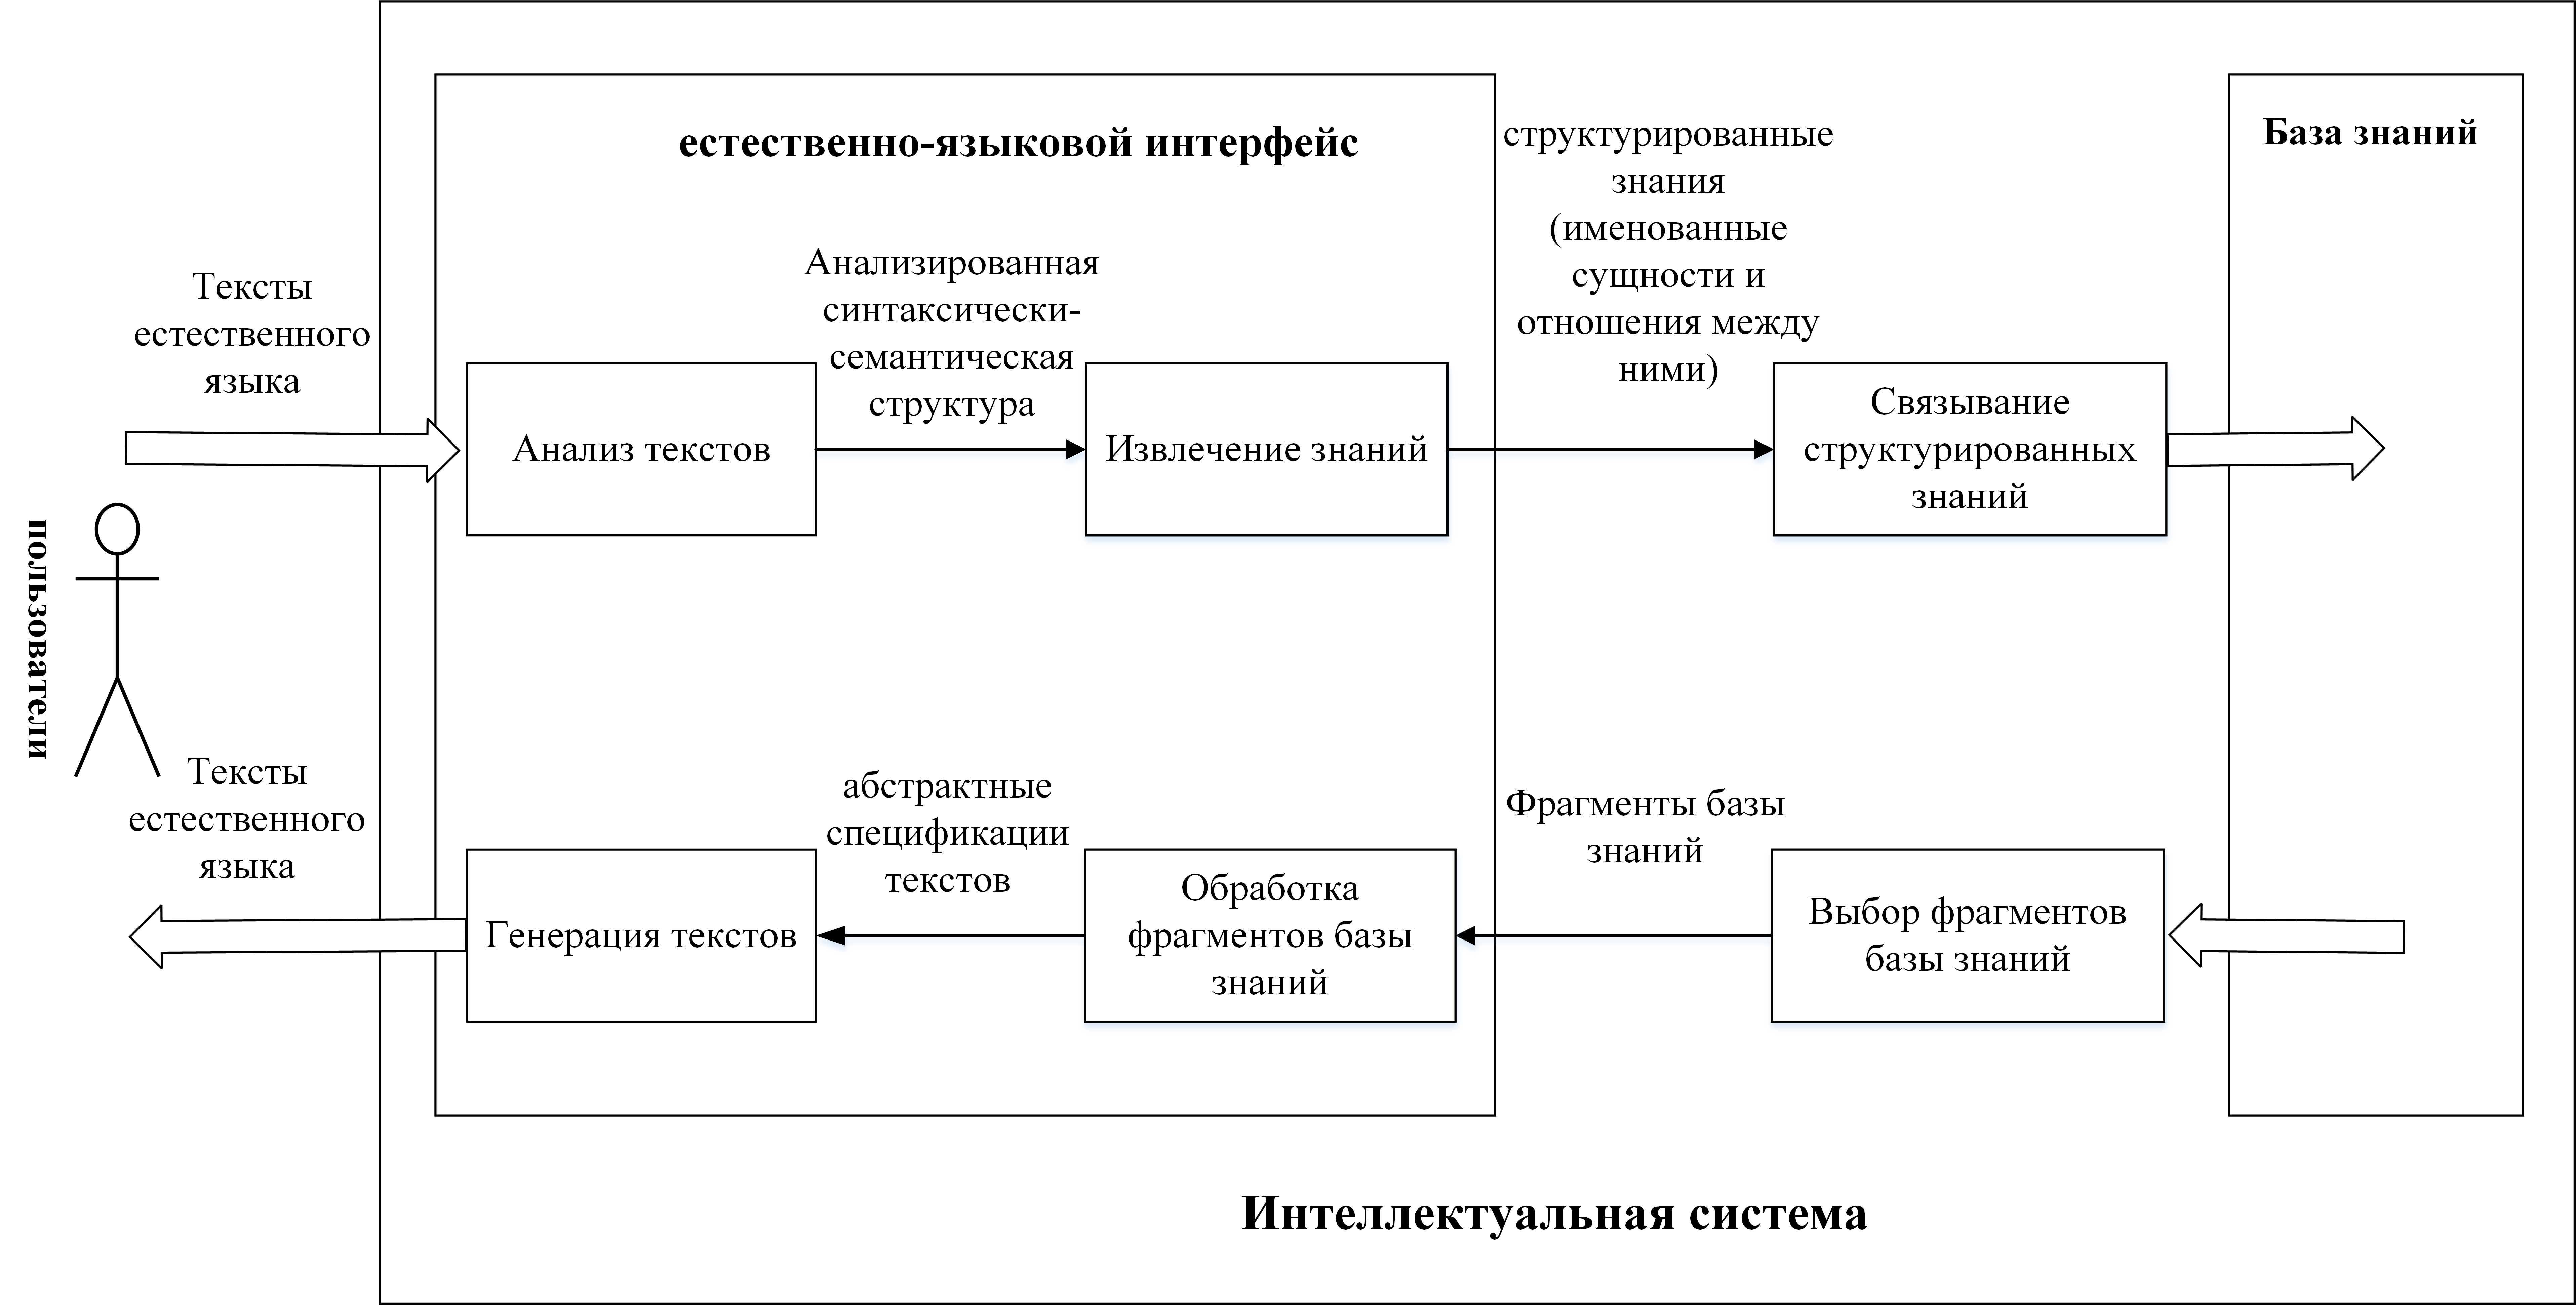
\includegraphics[scale=0.8,width=1.0\textwidth]{images/part4/chapter_chinese/schema1.png}
	\caption{Модульная схема вопросно-ответных систем, основанных на знаниях}
	\label{fig:schema-natural-interface}
\end{figure}

Современные вопросно-ответные системы в основном сосредоточены на обработке вопросительных предложений и поиске правильных ответов в базе знаний систем. Кроме того, генерация ответов вопросно-ответных системах часто напрямую выводит правильный фрагменты базы знаний в качестве ответов, которые неудобны для чтения пользователями. Генерация ответов может быть легко реализована в современных вопросно-ответных системах. В большинстве систем даже нет необходимости реализовывать  модули обработки фрагментов базы знаний и генерации текстов.

В нашей работе разработка естественно-языковых интерфейсов интеллектуальных систем ориентирована на решение следующих двух задач:
\begin{textitemize}
	\item преобразование входных текстов естественного языка (в частности
	повествовательные предложения) в фрагменты базы знаний интеллектуальных систем (приобретение/извлечение фактографических знаний (в основном именованных сущностей и отношений между ними));
	\item генерация текстов естественного языка (в частности
	повествовательные предложения) из фрагментов базы знаний интеллектуальных систем (генерация текстов естественного языка).
\end{textitemize}

Разработка естественно-языковых интерфейсов для современных интеллектуальных систем, основанных на знаниях, в общем случае требует рассмотрения следующих двух основных аспектов:
\begin{textitemize}
	\item типы обрабатываемого естественного языка, т. е. характеристики различных типов естественного языка;
	\item диапазон базы знаний интеллектуальных систем, т. е. широта знаний в базах знаний интеллектуальных систем.
\end{textitemize}

По статистике лингвистов, в мире существуют тысячи естественных языков. Однако в Интернете существуют лишь десятки естественных языков, которые широко используются конечными пользователями для общения, например, русский язык, английский язык, китайский язык и т. д. Каждый естественный язык имеет свои уникальные особенности. Таким образом, при использовании моделей, методики и средств для обработки текстов различных естественных языков необходимо учитывать соответствующие характеристики различных естественных языков. Кроме того, диапазон базы знаний также влияет на сложность разработки естественно-языковых интерфейсов. Например, базы знаний всемирного масштаба (см. \scncite{Liu2020}, см. \scncite{Abu2020}), в которых источники знаний ориентированы на Интернет, т. е. в базах знаний интеллектуальных систем хранятся знания здравого смысла (англ. commonsense knowledge). А базы знаний специализированные (см. \scncite{Xu2016}), в которых источники знаний ориентированы на различные энциклопедии (например, автомобильная энциклопедия, энциклопедия о фильмах, энциклопедия о разных дисциплинах (дискретная математика, история и другие) и т.д.), т. е. в базах знаний интеллектуальных систем хранятся конкретные отраслевые знания (т. е. знания об ограниченной предметной области). Общие базы знаний обращают внимание на широту хранимых знаний, подчеркивают интеграцию больше количества именованных сущностей по различным предметным областям и отношений между ними. Таким образом, общие базы знаний не обеспечивают высокую точность хранимых в них знаний (см. \scncite{Liu2020}). А также огромное количество именованных сущностей и отношений между ними в базе знаний приводит к высокой сложности поиска и обработки фрагментов базы знаний. В отличие от общих баз знаний, в специализированных базах знаний уделяется больше внимания глубине и точности хранящихся знаний, удовлетворяющих решение различных задач в интеллектуальных системах с низкой сложностью. 

В соответствии с двумя перечисленными выше аспектами, естественно-языковые интерфейсы интеллектуальных систем можно разделить на следующие формы:
\begin{textitemize}
	\item \textbf{интерфейс, не зависящий от конкретного естественного языка и конкретной предметной области.} В данном случае это означает, что интерфейс может обрабатывать тексты любых видов естественных языков, например, русский язык, арабский язык, английский язык и китайский язык и так далее, а также обрабатывать любую сложную структуру знаний, т. е. знания в базах знаний всемирного масштаба;
	\item интерфейс, зависящий от конкретного естественного языка, но не зависящий от конкретной предметной области. В этом случае интерфейс может анализировать только тексты определенного естественного языка и обрабатывать любую сложную структуру знаний;
	\item \textbf{интерфейс, не зависящий от конкретного естественного языка, но зависящий от конкретной предметной области.} В этом случае интерфейс может анализировать тексты любых видов естественных языков, обрабатывать тексты естественного языка, описывающие факты в конкретной предметной области. И специализированная база знаний является основой базы знаний данной интеллектуальной системы. Следует отметить, что описание фактов в разных предметных областях может использовать особенные виды предложений. Таким образом, обработка текстов естественного языка, описывающих факты в разных предметных областях (например, исторический текст, юридический текст, текст в дисциплинах), имеет разную степень сложности;
	\item \textbf{интерфейс, зависящий от конкретного естественного языка и зависящий от конкретной предметной области.} Данный интерфейс считается самым основным естественно-языковым интерфейсом в интеллектуальных системах. В этом случае интерфейсу нужно только анализировать тексты определенного естественного языка и обрабатывать легкую структуру знаний в специализированной базе знаний. 	
\end{textitemize}

Всем известно, что построение базы знаний всемирного масштаба является огромном проектом. А также база знаний всемирного масштаба в основном используется в Интернет ориентированных поисках, рекомендациях и вопросно-ответных задачах. Сценарий применения относительно единственно. Однако плотность знаний в специализированной базе знаний более высока, \textbf{интерфейс, не зависящий от конкретного естественного языка, но зависящий от конкретной предметной области} могут выполняться больше сценарии применения. 

В современных интеллектуальных системах отсутствует единая основа для разработки естественно-языковых интерфейсов, которая приводит к высокой сложности и трудоемкости разработки естественно-языковых интерфейсов. Как приобретение фактографических знаний, так и генерация текстов естественного языка считаются подзадачами обработки естественного языка. С точки зрения интеллектуальных систем, данные подзадачи представляют собой разновидности так называемых комплексных задач, решение которых до сих пор является актуальной темой исследований в области искусственного интеллекта. В целом, решение данных подзадач требует сочетание различных типов лингвистических знаний и интеграция различных моделей решения задач по обработке естественного языка. Однако в разработке естественно-языковых интерфейсов отсутствует единый принцип для интеграции различных типов лингвистических знаний и моделей решения задач для обработки естественного языка.

На данный момент существует большое количество методов для приобретения фактографических знаний и генерации текстов естественного языка, которые в основном можно разделить на два направления:
\begin{textitemize}
	\item методы на основе правил и лингвистических знаний;
	\item методы машинного обучения, основанные на математической статистике и теории информации.
\end{textitemize}

Первое направление предполагает разработку систем на основе лингвистических правил, соответствующих грамматике определенного естественного языка, сформулированных вычислительными лингвистами и другими лингвистами. В данных системах могут строиться правила извлечения, шаблоны для генерации текстов и другие на основе лингвистических знаниях для извлечения фактографических знаний и генерации текстов. 

Под извлечением фактографических знаний понимается приобретение фактографической информации, такой как понятия, именованные сущности, отношения между ними, а также определенный тип событий из текстов естественного языка, причем извлеченные результаты формализуются в виде внутреннего языка представления знаний интеллектуальных систем (например, RDF и другие). По сути, с точки зрения построения базы знаний интеллектуальных систем, отношения между именованными сущностями рассматриваются как особенные сущности, которые извлекаются из текстов естественного языка. 

Задача извлечения фактографических знаний из текстов естественного языка можно разделить на два направления по сфере извлеченной области:
\begin{textitemize}
	\item извлечение фактографических знаний из закрытых областей;
	\item извлечение фактографических знаний из открытых областей.
\end{textitemize}

Задача извлечения фактографических знаний из закрытых областей часто требует заранее определенных типов именованных сущностей и отношений между ними. Однако в области извлечения фактографических знаний может быть не существуют ограниченные и определенные типы именованных сущностей и отношений между ними. Таким образом, цель извлечения фактографических знаний из открытой области состоит в том, чтобы извлекать различные наборы именованных сущностей и отношений между ними из массивных и разнородных корпусов текстов естественного языка без требований заранее заданного словаря для установления типа данных именованных сущностей и отношений между ними.

Извлечение фактографических знаний из открытых областей напрямую определяет относительные слова или словосочетания в текстах, анализируя тексты естественного языка (в частности, предложения), чтобы реализовать моделирование классификаций именованных сущностей и отношений между ними без необходимости заранее определений категорий данных именованных сущностей и отношений между ними.  Например, система CORE (см. \scncite{Tseng2014}) использует ряд технологий обработки китайского языка, таких как сегментация слов, автоматическая морфологическая разметка (POS tagging), скорректированная и подходящая для текстов китайского языка, синтаксический анализ, семантический анализ и правила извлечения для извлечения именованных сущностей и отношений между ними из текстов китайского языка. В данных системах построение правил вручную неэффективно, а также построенные правила сложно переносятся в других интеллектуальных системах для обработки китайского языка.

Для генерации текстов естественного языка существует классическая конвейерная архитектура (см. \scncite{Gatt2017}), на основе которой большинство систем генерации текстов имеет три основных модуля:
\begin{textitemize}
	\item планирование содержания текстов: уточнение, какая информация из входных данных будет включена в сгенерированные тексты, и как она будет организована;
	\item микро-планирование: решение, каким образом выбранная информация будет реализована языковыми средствами в виде предложений на естественном языке. В этом процессе преобразования информации в лингвистические выражения, обычно представлены предложения в виде структур семантических и/или синтаксических отношений;
	\item реализация на естественном языке: производство грамматически правильных предложений естественного языка.
\end{textitemize}

В самом начале системы генерации текстов широко используют шаблоны и грамматические правила, построенные исследователями для генерации текстов естественного языка. Система NaturalOWL (см. \scncite{Androutsopoulos2013}) представляет собой классическую систему генерации естественного языка, которая рационально применяет шаблоны и лингвистические правила для генерации текстов естественного языка (в основном английский язык), описывающих фрагменты OWL онтологий. Однако, в данной системе не предоставлена модель семантического представления знаний, что позволяет представлять различные виды знаний в единой базе знаний, включая лингвистические знания, логический вывод на онтологиях лингвистики и шаблоны, построенные на онтологиях. 

Второе направление, широко применяемое в настоящее время в современных интеллектуальных системах, предполагает использование различных моделей машинного обучения, основанных на математической статистике и теории информации, которые направлены на моделирование текстов естественного языка.

В настоящее время подходы, основанные на моделей машинного обучения (в частности модели нейронных сетей), в основном используются для извлечения фактографических знаний из закрытых областей, например, серия моделей предварительной подготовки BERT (см. \scncite{Devlin2018}), GPT (см. \scncite{Brown2020}) и т.д. Использование моделей нейронных сетей всегда требует дорогие аппаратные оборудования и очень больших корпусов данных, которые аннотируются вручную человеком. Более того, производительность данных моделей сильно зависит от качества аннотирования обучающих выборок. 

Для обучения моделей нейронных сетей, ориентированных на генерацию текстов естественного языка, обучающие данные обычно представляются в виде пары входов (фрагменты базы знаний) и выходов (тексты естественного языка) (см. \scncite{Moryossef2019}). В последние годы в проекте WebNLG (см. \scncite{Gardent2017}) основная задача направлена на разработку нейронных генераторов с помощью моделей нейронных сетей для решения задач генерации текстов. Для разработки нейронных генераторов команда проекта предоставляет обучающие данные, которые состоят из пар Данные/Тексты для английского языка и русского языка, где данные представляют собой фрагменты базы знаний в виде RDF, извлеченных из DBpedia (см. \scncite{Lehmann2015}). Для других естественных языков, таких как китайский язык, наборы данных для обучения генераторов отсутствуют, хотя и существуют несколько известных баз знаний на китайском языке в области обработки китайского языка, например, CN-DBpedia (см. \scncite{Xu2017}), zhishi.me (см. \scncite{Niu2011}) и другие, которые могут предоставлять фрагменты базы знаний в виде RDF. Построение высококачественных наборов данных для китайского языка является трудоемким и трудно-затратным процессом. 

Разработанные системы извлечения фактографических знаний из открытых областей и разработанные различные генераторы были успешно применены в различных областях. Тем не менее, к проблемам существующих решений к разработке естественно-языкового интерфейса и обработке естественного языка в естественно-языковом интерфейсе можно отнести:
\begin{textitemize}
	\item отсутствие единой основы в процессе разработки естественно-языковых интерфейсов и интеграция различных компонентов (база знаний по обработке естественного языка, компонент для извлечения фактографических знаний, компонент для генерации текстов), разработанных разными разработчиками, приводит к сложной трудоемкости и невозможности распараллеливания разработки естественно-языковых интерфейсов;
	\item отсутствие возможности использования единой основы для представления различных видов лингвистических знаний в единой базе знаний для обработки естественного языка;
	\item отсутствие подходов к возможности интеграции различных моделей решения задач для извлечения фактографических знаний и генерации текстов естественного языка;
	\item для приобретения фактографических знаний в существующих онтологических подходах построенные правила часто применимы только в извлечениях фактографических знаний из закрытых областей и ограниченных условиях;
	\item качество извлеченных фактографических знаний и генерируемых текстов зависит от искусственно сконструированных шаблонов и правил, но построение конкретных шаблонов и правил для текстов различных естественных языков является чрезвычайно сложной и трудоемкой задачей из-за отсутствия единой основы;
	\item для приобретения фактографических знаний и генерации текстов, большие языковые модели на основе моделей нейронных сетей используется для обработки естественного языка. Используя модели нейронных сетей, необходимо дорогие аппаратные оборудования и высококачественные согласованные учебные корпусы, которые  крайне сложно получить и построить.
\end{textitemize}

Построение единой семантической модели естественно-языковых интерфейсов осуществляется на основе \scnkeyword{Технологии OSTIS} (см. \scncite{Golenkov2014a}), что обеспечивает единую основу для эффективного объединения различных лингвистических знаний, включая правила извлечения, шаблоны для генерации текстов и другие лингвистические знания по обработке естественного языка, а также глубокой интеграции различных моделей решения задач (например логические модели на основе правил, модели нейронных сетей и другие) для решения задач преобразования текстов естественного языка в фрагменты базы знаний и генерации текстов естественного языка из фрагментов базы знаний в естественно-языковых интерфейсах (рисунок \textit{\nameref{fig:structure-sc-model-natural-interface}}). Системы, построенные по указанной Технологии OSTIS, названы ostis-системами.

\begin{figure}[H]
	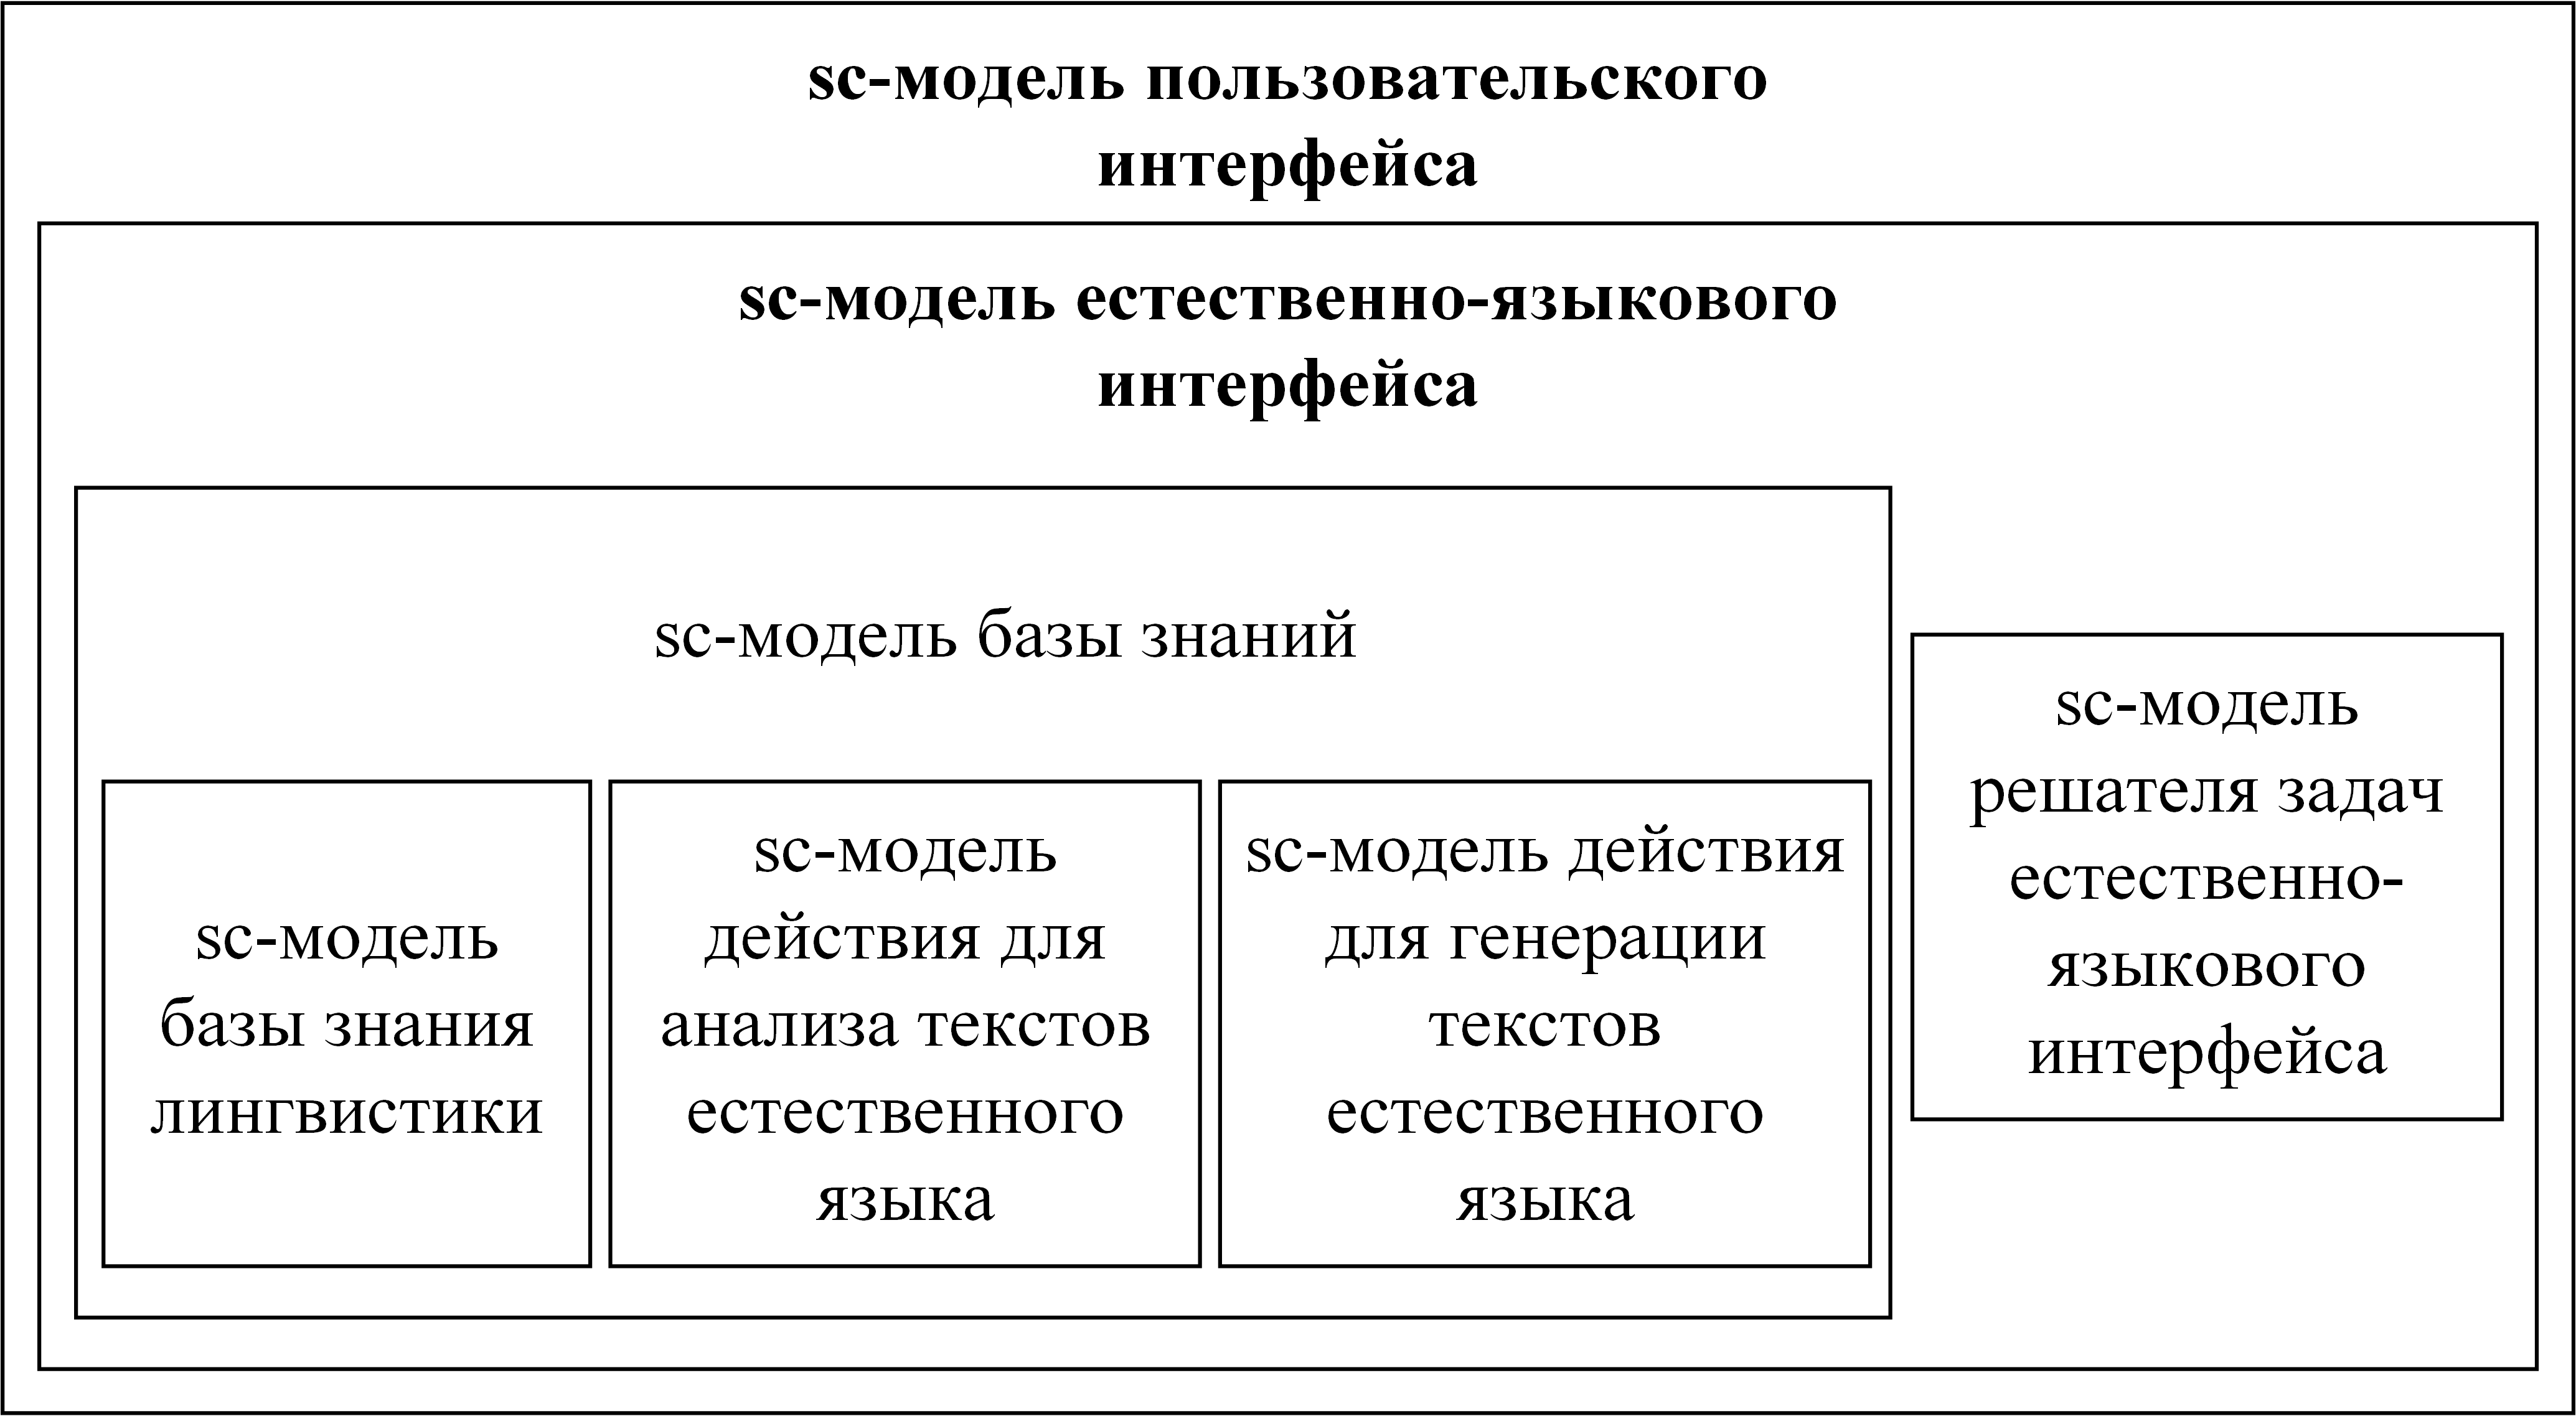
\includegraphics[scale=0.8,width=1.0\textwidth]{images/part4/chapter_chinese/structure_interface.png}
	\caption{Общая структура sc-модели естественно-языковых интерфейсов ostis-систем}
	\label{fig:structure-sc-model-natural-interface}
\end{figure}

Единая семантическая модель естественно-языковых интерфейсов интеллектуальных систем по конкретной предметной области позволяет, в принципе, потенциально реализовать преобразование текстов различных естественных языков в фрагменты базы знаний и генерации текстов различных естественных языков из фрагментов базы знаний, просто сложность построения базы знаний по обработке конкретного естественного языка, объединяющей различные виды лингвистических знаний, будет разным в зависимости от особенностей конкретного естественного языка, а также потребуются определенные дополнительные sc-агенты, входящие в решатели задач естественно-языкового интерфейса по особенностям конкретного естественного языка, интегрирующие логические модели на основе правил и модели нейронных сетей для обработки текстов конкретного естественного языка.

\subsection{SC-модель базы знаний лингвистики}
База знаний лингвистики содержит формальное описание необходимых лингвистических знаний для анализа текстов естественного языка и генерации текстов естественного языка (см. \scncite{Qian2020}). Соответствующие онтологии обеспечивают формальное описание понятий, используемых для представления таких лингвистических знаний на различных уровнях от базовых слов до синтаксических или семантических структур текстов естественного языка по обработке естественного языка. Лингвистические теории, предложенные лингвистами, обеспечивают теоретическую основу для построения SC-модели базы знаний лингвистики. 

В рамках \scnkeyword{Технологии OSTIS} sc-модель базы знаний рассматривается, как иерархическая система выделенных предметных областей и соответствующих им онтологий (см. \scncite{Davydenko2018}). Основная иерархия SC-модели базы знаний лингвистики, используемая для решения задач преобразований текстов естественного языка в фрагменты базы знаний и генерации текстов естественного языка из фрагментов базы знаний:
\begin{SCn}
	\scnheader{SC-модель базы знаний лингвистики}
	\scnidtf{SC-модель лингвистической базы знаний}
	\scnidtf{SC-модель базы знаний по обработки естественного языка}
	\scnidtf{SC-модель базы знаний естественно-языковых интерфейсов}
	\begin{scnrelfromset}{декомпозиция раздела}
		\scnitem {Предметная область лексического анализа}
		\scnitem {Предметная область синтаксического анализа}
		\scnitem {Предметная область семантического анализа}
	\end{scnrelfromset}
\end{SCn}

Предметная область лексического анализа включает в себя ряд онтологий для лексического анализа, которые описывают характеристики слов и синтаксические функции слов, части речи и т.д. В обработке естественного языка \textit{слово} -- это наименьшая единица естественного языка, несущая семантику, которая служит для наименования объектов, их качеств, характеристик и взаимодействий, а также для служебных целей. \textit{Номинативная единица} -- устойчивая последовательность комбинаторных вариантов лексем.
\begin{SCn}
	\scnheader{текст естественного языка}
	\scnsubset{файл}
	\scnheader{слово}
	\scnsubset{файл}
	\scnheader{номинативная единица}
	\scnsubset{файл}
\end{SCn} 

В русском, английском или других европейских языках структура слова изучается в рамках морфологии. Лексема рассматривается для описания особенностей слов в европейских языках, обладающих признаком морфологической парадигмы. В китайском языке из-за письменной традиции (текст китайского языка состоит потока иероглифов без естественных пробелов), единица сегментации рассматривается как наименьшая единица для обработки текстов китайского языка, был предложен в государственном стандарте «Стандарт сегментации слов современного китайского языка, используемый для обработки информации». 
\begin{SCn}
	\scnheader{единица сегментации}
	\scnidtfdef{базовая единица для обработки китайского языка с определенными семантическими или грамматическими функциями}
	\scnsubset{файл}
\end{SCn}

Стоит отметить, что описание единица сегментации ориентировано на компьютерную обработку китайского языка и не полностью совпадает с описанием слов в китайской лингвистике.

\textit{Часть речи} -- это категория слов естественного языка, определяемая морфологическими, синтаксическими и семантическими особенностями. Хотя часть речи, предложенная для анализа текстов европейских языков, не полностью подходит к анализу текстов китайского языка, но часть речи может частично решить задачи в обработке китайского языка. В 2001 г. был предложен государственный стандарт «Принцип частеречной разметки
в обработке современной китайской информации», устанавливающий конкретный стандарт морфологической разметки. 
\begin{SCn}
	\scnheader{часть речи по обработке китайского языка}
	\scnrelto{семейство подмножеств}{единица сегментации}
	\scnhaselement{существительное}
	\scnhaselement{прилагателбное}
	\scnhaselement{глагол}
	\scnhaselement{наречие}
	\scnhaselement{идиома}
	\scnhaselement{союз}
	\scnhaselement{географическое название}
	\scnhaselement{модальный глагол}
\end{SCn}

Категории в части речи по обработке китайского языка построены с учета особенности китайского языка на лингвистических теорий европейских языков. 

Предметная область синтаксического анализа описывает характеристики синтаксиса естественного языка, функциональные характеристики синтаксических компонентов (таких как, слово, словосочетание, предложение и т.д.). Среди них в области обработки естественного языка предложение всегда рассматривается как наименьшая единица исследования. Анализ предложений является важным промежуточным этапом, связывающим анализ всех текстов и анализ отдельных слов. 

В зависимости от особенностей китайского языка существуют соответствующие различные синтаксические структуры для предложений китайского языка.

\begin{SCn}
	\scnheader{предложение китайского языка}
	\begin{scnrelfromset}{разбиение}
		\scnitem{простое предложение}
		\scnidtfdef{предложение содержит в себе одну предикативную единицу}
		\scnitem{сложное предложение}
		\scnidtfdef{предложение содержит в себе больше одну предикативную единицу}
	\end{scnrelfromset}
\end{SCn}

\begin{SCn}
	\scnheader{предложение китайского языка}
	\begin{scnrelfromset}{разбиение}
		\scnitem{предложение с подлежащим и сказуемым}
		\scnitem{предложение без подлежащего и сказуемого}
		\scnitem{предложение с особенным знаком алфавита синтаксиса}
	\end{scnrelfromset}
\end{SCn}

\begin{SCn}
	\scnheader{член предложения\scnrolesign}
	\begin{scnrelfromset}{разбиение}
		\scnitem{главный член предложения\scnrolesign}
		\begin{scnindent}
			\begin{scnrelfromset}{разбиение}
				\scnitem{подлежащее\scnrolesign}
				\scnitem{сказуемое\scnrolesign}
				\scnitem{прямое дополнение\scnrolesign}
			\end{scnrelfromset}
		\end{scnindent}
		\scnitem{второстепенный член предложения\scnrolesign} 
		\begin{scnindent}
			\begin{scnrelfromset}{разбиение}
				\scnitem{косвенное дополнение\scnrolesign}
				\scnitem{определение\scnrolesign}
				\scnitem{обстоятельство\scnrolesign}
			\end{scnrelfromset}
		\end{scnindent}
	\end{scnrelfromset}
\end{SCn}

\textit{Член предложения\scnrolesign} -- рольное отношение, связывающее декомпозицию текста с файлом, содержимое которого (отдельное слово или словосочетание из текста) играет в делительном тексте определенную синтаксическую роль (см. \scncite{Hardzei2022}).

\begin{SCn}
	\scnheader{отношение зависимости*}
	\scnidtfdef{описание зависимости отдельных слов или словосочетаний в предложении друг от друга.}
	\scnhaselement{суъбект*}
	\scnhaselement{объект*}
	\scnhaselement{дополнение глагола*}
	\scnhaselement{определитель*}
	\scnhaselement{атрибут*}
	\scnhaselement{модификатор*}
\end{SCn}

На основе теории синтаксиса грамматики зависимостей для китайского языка, \textit{отношение зависимости*} -- отношение, связывающее делительные два файла из предложения естественного языка направленными связями, содержимое которых отдельно называется исходным словом (англ. head), которое часто играет роль сказуемое' в предложении, и целевым словом (англ. depedent). Каждое целевое слово несет синтаксическую функцию по зависимости к исходному слову. В общем случае, при синтаксическом анализе предложений китайского языка глаголы (или глагольные словосочетания) (также называется конечные глаголы, исходные слова) часто считаются структурными центрами придаточной структуры. Все остальные синтаксические единицы (слова или словосочетания) прямо или косвенно связаны с глаголом посредством направленных связей (т. е. направление с глаголом до других синтаксических единиц). В области обработки китайского языка были предложены Харбинским политехническим университетом ряды отношений зависимости (см. \scncite{Liu2006}).

В логической онтологии предметной области синтаксического анализа можно описать ряды логических определений и логических утверждений для обработки предложений. В виде логических утверждений могут быть построены правила или шаблоны для приобретения фактографических знаний и генерации текстов, которые могут использоваться решателями задач для решения конкретных задач в естественно-языковых интерфейсах.
\begin{figure}[H]
	\centering
	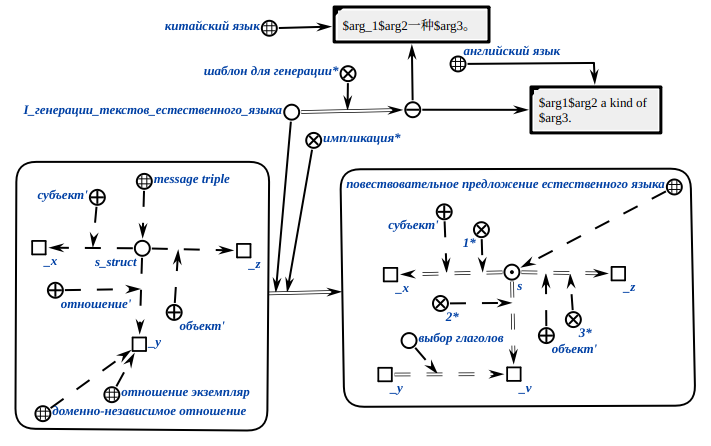
\includegraphics[scale=0.8]{images/part4/chapter_chinese/ruleGeneration.png}
	\caption{Логическое утверждение про генерации предложения на основе шаблона}
	\label{fig:template-generation}
\end{figure}

На рисунке \textit{\nameref{fig:template-generation}} указано на языке SCg, что эвристическое правило, используемое для генерации текстов естественного языка. Как показано на рисунке, если установлено, что отношение в ``message triple'' принадлежит к доменно-независимое отношение, то шаблон используется для генерации текстов. Компоненты субъект и объект в ``message triple'' заполняются в параметр 1 и параметр 3 в шаблоне, соответственно, а затем соответствующий глагол (или глагольное словосочетание) для отношения в ``message triple'' выбирается в качестве параметра 2 в шаблоне. Понятия ``message triple'' и доменно-независимых отношений будут показаны ниже.

Предметная область семантического анализа описывает семантические характеристики слов и семантическую структуру предложений естественного языка, функциональные характеристики семантики компонентов (слов, словосочетаний и предложений и т.д.), семантические роли, правила семантического анализа и так далее.

Предметная область семантического анализа на уровне лексемы описывает семантические классификации общих базовых понятий, выраженных лексемой, или привязку лексемы к отдельным сущностям. Предметная область была построена на основе различных типов баз семантических знаний о естественном языке, используемых для семантического анализа на уровне лексемы или предложений, например, WordNet, ConcetpNet, The Semantic Knowledge base of Modern Chinese (см. \scncite{Wang2006}), TAPAZ-2 и т. д.

\begin{SCn}
	\scnheader{семантические категории в естественном языке}
	\scnhaselement{семантические категории для глаголов}
	\scnhaselement{семантические категории для существительных}
	\scnhaselement{семантические категории для прилагателбных}
	\scnhaselement{семантические категории для наречий}
\end{SCn}


\begin{SCn}
	\scnheader{участник воздействия*}
	\scnidtf{участник акции*}
	\scnidtf{участник события*}
	\scniselement{неролевое отношение}
	\scnrelfrom{первый домен}{индивид}
	\scnrelfrom{вторый домен}{акция}
	\begin{scnrelfromset}{разбиение}
		\scnitem {субъект*}
		\begin{scnindent}
			\begin{scnrelfromset}{разбиение}
				\scnitem {инициатор*}
				\scnitem {вдохновитель*}
				\scnitem {распространитель*}
				\scnitem {вершитель*}
			\end{scnrelfromset}
		\end{scnindent}
		\scnitem {объект*}
		\begin{scnindent}
			\begin{scnrelfromset}{разбиение}
				\scnitem {покрытие*}
				\scnitem {корпус*}
				\scnitem {прослойка*}
				\scnitem {сердцевина*}
			\end{scnrelfromset}
		\end{scnindent}
	\end{scnrelfromset}
\end{SCn}

\textit{Индивид} является разновидностью стереотипа как отдельной сущности, которая представляет собой  экземпляр конкретных понятий. 

\textit{Участник действия*} -- это неролевое отношение, которое связывает действие с индивидом, участвующим в нем, в определенной степени его можно рассматривать как семантическую роль действия. Соответственно действие обычно выражается глаголом или глагольной фразой в предложении.

В свою очередь, аналогично предметная область семантического анализа на уровне предложения описывает семантическую структуру предложений, семантические отношения между компонентами (словами, словосочетаниями и т.д.) в предложении, а также семантические отношения между предложениями в текстах. Некоторые открытые базы знаний, например, TAPAZ-2, PropBank и другие, послужили основой для построения данной предметной области.

В sc-модели естественно-языковых интерфейсов база знаний лингвистики просто предоставляет синтаксические лингвистические знания решателями задач для решения соответствующих задач в естественно-языковых интерфейсах. Кроме того, естественно-языковые интерфейсы должны иметь динамическую возможность выполнять некоторые действия для решения задач по обработке естественного языка в естественно-языковых интерфейсах. 
\begin{SCn}
	\scnheader{действие для естественно-языковых интерфейсов}
	\begin{scnrelfromset}{декомпозиция}
		\scnitem{действие для преобразования текстов естественного языка в фрагменты базы знаний}
		\scnitem{действие для генерации текстов естественного языка из фрагментов базы знаний}
	\end{scnrelfromset}
\end{SCn}

\begin{SCn}
	\scnheader{действие для преобразования текстов естественного языка в фрагменты базы знаний}
	\begin{scnrelfromset}{декомпозиция}
		\scnitem{действие для разбиений текстов на отдельные единицы}
		\scnitem{действие для разметки отдельных единиц}
		\scnitem{действие для синтаксического анализа}
		\scnitem{действие для семантического анализа}
		\scnitem{действие для формирования структур фактографических знаний}
		\scnitem{ействие для связываний фактографических знаний в базу знаний}
		\scnitem{действие для установления противоречий}
		\scnitem{действие для устранений противоречий}
	\end{scnrelfromset}
\end{SCn}

\begin{SCn}
	\scnheader{действие для генерации текстов естественного языка из фрагментов базы знаний}
	\begin{scnrelfromset}{декомпозиция}
		\scnitem{действие для локализации фрагментов базы знаний}
		\scnitem{действие для преобразований фрагментов в стандартные базовые sc-конструкции}
		\scnitem{действие для установления проективных базовых sc-конструкций}
		\scnitem{действие для преобразований проективных sc-конструкций в message triple}
		\scnitem{действие для генерации результирующих текстов из message triple}
	\end{scnrelfromset}
\end{SCn}

С точки зрения генерации текста из фрагментов базы знаний ostis-системы, следует отметить, что ``message triple'' представляет собой вид упорядоченной последовательности текстов естественного языка, представленной в виде <субъект, отношение, объект>, где субъект -- это всегда идентификатор множества sc-узлов, обозначающих понятия, не являющиеся отношениями, или элемент данного множества sc-узлов; отношение -- идентификатор множества sc-узлов, обозначающих ролевые или неролевые отношения, которые указывает на связку, соединяющую субъект и объект; объект -- идентификатор множества sc-узлов, обозначающих понятия, не являющиеся отношениями, или элемент данного множества sc-узлов. У состава sc-структур (и sc-конструкций) есть sc-дуги, которые имеют конкретные значения. Таким образом, sc-структуры (и sc-конструкции) с sc-дугами нужны преобразовать в ``message triple'' в текстовом виде, которые легче представляют в виде текстов естественного языка.

В процессе генерации, ``message triple'' рассматривается как промежуточное преобразование между sc-структурой и результирующим текстом, главным образом потому что данный вид упорядоченной последовательности текстов легче выразить в виде текстов естественного языка (в основном предложения), используя либо модели шаблонов или правил, либо современные модели нейронных сетей. 

\subsection{SC-модель решателя задач естественно-языковых интерфейсов}
Для реализации естественно-языковых интерфейсов ostis-систем необходимо разработать SC-модель решателя задач естественно-языковых интерфейсов, в рамках которой SC-модель решателя задач рассматривается как иерархическая система агентов (см. \scncite{Shunkevich2017}), способного выполнять вышеупомянутые действия в sc-памяти для решения задач анализа текстов естественного языка и генерации текстов естественного языка в естественно-языковых интерфейсах.
\begin{SCn}
	\scnheader{SC-модель решателя задач естественно-языковых интерфейсов}
	\scnidtf{SC-модель решателя задач по обработке естественного языка}
	\begin{scnrelfromset}{декомпозиция}
		\scnitem{SC-модель решателя задач анализа текстов естественного языка}
		\scnitem{SC-модель решателя задач генерации текстов естественного языка}
	\end{scnrelfromset}
\end{SCn}

В естественно-языковых интерфейсах SC-модель решателя задач анализа текстов естественного языка предназначена для решения задач извлечения фактографических знаний (как правило, именованные сущности и отношения между ними) из текстов естественного языка в открытых областях.

\begin{SCn}
	\scnheader{SC-модель решателя задач анализа текстов естественного языка}
	\scnidtf{SC-модель решателя задач приобретения фактографических знаний}
	\begin{scnrelfromset}{декомпозиция абстрактного sc-агента}
		\scnitem{Абстрактный sc-агент лексического анализа}
		\begin{scnindent}
			\begin{scnrelfromset}{декомпозиция абстрактного sc-агента}
				\scnitem {Абстрактный sc-агент разбиения текстов на отдельные единицы}
				\scnitem {Абстрактный sc-агент разметки отдельных единиц}
			\end{scnrelfromset}
		\end{scnindent}
		\scnitem{Абстрактный sc-агент синтаксического анализа}
		\scnitem{Абстрактный sc-агент семантического анализа}
		\scnitem{Абстрактный sc-агент извлечения структур фактографических знаний в базу знаний}
		\begin{scnindent}
			\begin{scnrelfromset}{декомпозиция абстрактного sc-агента}
				\scnitem {Абстрактный sc-агент формирования структур фактографических знаний}
				\scnitem {Абстрактный sc-агент связывания фактографических знаний в базу знаний}
				\scnitem {Абстрактный sc-агент установления противоречий}
				\scnitem {Абстрактный sc-агент устранения противоречий}
			\end{scnrelfromset}
		\end{scnindent}
		\scnitem{Абстрактный sc-агент логического вывода}
	\end{scnrelfromset}
\end{SCn}

\textit{\textbf{Абстрактный sc-агент разбиения текстов на отдельные единицы}} -- группы агентов, реализующие механизмы декомпозиции входных текстов естественного языка на лексические единицы. Компоненты (слова, словосочетания, предложения и другие) входных текстов естественного языка могут быть определены по определенному стандарту конкретного естественного языка.

\textit{\textbf{Абстрактный sc-агент разметки отдельных единиц}} -- коллектив агентов, реализующих механизмы разметки раздельных лексических единиц по определенному принципу конкретного естественного языка, устанавливающему конкретный стандарт разметки. 

\textit{\textbf{Абстрактный sc-агент синтаксического анализа}} -- коллектив агентов, реализующих механизмы построения синтаксической структуры входных текстов естественного языка.

\textit{\textbf{Абстрактный sc-агент семантического анализа}} -- коллектив агентов, реализующих механизмы построения семантической структуры входных текстов естественного языка.

\textit{\textbf{Абстрактный sc-агент извлечения структур фактографических знаний в базу знаний}} -- коллектив агентов, реализующих механизмы интеграции структур фактографических знаний в базу знаний ostis-систем по конкретной предметной области.

\textit{\textbf{Абстрактный sc-агент формирования структур фактографических знаний}} -- коллектив агентов, реализующих механизмы, которые устанавливают структуры фактографических знаний во входных текстах естественного языка (т.е. установление именованных сущностей и отношений между ними).

\textit{\textbf{Абстрактный sc-агент связывания фактографических знаний в базу знаний}} -- коллектив агентов, реализующих механизмы связывания каждого элемента фактографических знаний в базу знаний ostis-систем по конкретной предметной области, включая наполнение экземпляров понятий с использованием именованных сущностей, сопоставление именованных сущностей и отношений между ними в базе знаний ostis-систем по конкретной предметной области.

В процессе отображения структур знаний в базу знаний, при сравнении структур знаний, извлеченных в результате анализа входных текстов естественного языка, с знаниями, хранящимися в базе знаний ostis-систем по конкретной предметной области, \textit{\textbf{Абстрактный sc-агент установления противоречий}} -- коллектив агентов, реализующих механизмы установления противоречий, например, для определенной именованной сущности во входных текстах естественного языка может быть существует несколько соответствующих экземпляров понятий. 

\textit{\textbf{Абстрактный sc-агент устранения противоречий}} -- коллектив агентов, реализующих механизмы устранения противоречий, в случае обнаружения противоречий. 

\textit{\textbf{Абстрактный sc-агент логического вывода}} -- коллектив агентов, реализующих механизмы, которые используют логические правила, записанные средствами SC-кода, для синтаксического анализа, семантического анализа и также извлечения структур фактографических знаний. Таким образом, данный агент может взаимодействовать с агентами синтаксического, семантического анализа и агентом извлечения структур фактографических знаний.

При решении задач генерации текстов SC-модель решателя задач генерации текстов естественного языка разработана на основе классического конвейера. Хотя разработка SC-модели данного решателя основана на классическом конвейере, разработка конкретных составов решателя может быть гибка за счет использования многоагентного подхода (см. \scncite{Qian2022}). Для генерации текстов конкретного естественного языка, составы решателя задач можно соответствующим образом легко модифицировать.
\begin{SCn}
	\scnheader{SC-модель решателя задач генерации текстов естественного языка}
	\begin{scnrelfromset}{декомпозиция абстрактного sc-агента}
		\scnitem{Абстрактный sc-агент локализации фрагмента базы знаний}
		\scnitem{Абстрактный sc-агент планирования структуры текстов}
		\scnitem{Абстрактный sc-агент микро-планирования}
		\scnitem{Абстрактный sc-агент реализации текстов естественного языка}
	\end{scnrelfromset}
\end{SCn}

\begin{SCn}
	\scnheader{Абстрактный sc-агент локализации фрагмента базы знаний}
	\begin{scnrelfromset}{декомпозиция абстрактного sc-агента}
		\scnitem{Абстрактный sc-агент локализации sc-структуры в базе знаний}
		\scnitem{абстрактный sc-агент разделения конкретной sc-структуры на базовые стандартные sc-конструкции}
		\scnitem{Абстрактный sc-агент установления конкретных проектных sc-конструкций}
		\scnitem{Абстрактный sc-агент преобразования конкретных sc-конструкций в соответствующие им message triple}
	\end{scnrelfromset}
\end{SCn}

\textit{\textbf{Абстрактный sc-агент локализации sc-структуры в базе знаний}} -- группа агентов, предоставляющих поиск sc-структуры из базы знаний ostis-систем по конкретной предметной области, составляющего из sc-конструкций стандартного вида, из которых будем преобразовывать тексты естественного языка. С точки зрения генерации текстов, на этом этапе, по сути, определяется, о чем мы хотим поговорить. 

\textit{\textbf{Абстрактный sc-агент разделения конкретной sc-структуры на базовые стандартные sc-конструкции}} -- группа агентов, реализующих механизмы декомпозиции поисковой sc-структуры на базовые стандартные sc-конструкции, которые могут быть переведены в ``message triple''. 

В некоторых случаях разделенные базовые sc-конструкции из sc-структуры являются избыточными, т.е. не все разделенные базовые sc-конструкции нужно преобразовывать в ``message triple'', а затем в тексты естественного языка, а некоторые sc-конструкции не являются той информацией, которую ожидают пользователи. Таким образом, естественно-языковой интерфейс требует окончательного выбора некоторых среди разделенных sc-конструкций в качестве проектных sc-конструкций, предоставляющих максимально полезную информацию пользователям, и даже подходящую для пользователей (для разных пользователей нужно предоставлять сгенерированные тексты различных стилей, например, для специалистов нужно использовать специальные термины в сгенерированных текстах). 

\textit{\textbf{Абстрактный sc-агент установления конкретных проектных sc-конструкций}} -- группа агентов, реализующих механизмы установления подходящих конкретных sc-конструкций, предоставляющих информацию пользователям и возможно удовлетворяющих конкретных пользователей. 

\textit{\textbf{Абстрактный sc-агент преобразования конкретных sc-конструкций в соответствующие им message triple}} -- группа агентов, реализующих механизмы перевода выбранных конкретных sc-конструкций в соответствующие ``message triple''.

\textit{\textbf{Абстрактный sc-агент планирования структуры текстов}} -- группа агентов, реализующих функцию структурирования сгенерированных текстов, т.е. установления упорядоченности ``message triple'', в данной упорядоченности ``message triple'' будут представлены в сгенерированных текстах. 
\begin{SCn}
	\scnheader{Абстрактный sc-агент планирования структуры текстов}
	\begin{scnrelfromset}{декомпозиция абстрактного sc-агента}
		\scnitem{Абстрактный sc-агент упорядочения message triple}
		\scnitem{Абстрактный sc-агент упорядочения именованных сущностей в каждом message triple}
	\end{scnrelfromset}
\end{SCn}

В общем случае, в базе знаний ostis-систем в качестве идентификаторов sc-элементов чаще всего используются имена (термины) соответствующих сущностей, представленные отдельными словами или словосочетаниями на различных естественных языках, но также могут использоваться иероглифы на китайском языке. Таким образом, в качестве идентификаторов (названий, терминов) именованных сущностей в ``message triple'' можно прямо использовать в сгенерированных текстах естественного языка. 

\textit{\textbf{Абстрактный sc-агент микро-планирования}} -- группа агентов, реализующих механизмы превращения ``message triple'' в абстрактные спецификации предложений естественного языка, которые варьируются в зависимости от систем генерации естественного языка, например, текстовые шаблоны с частично незаполненными слотами, которые будут заполнены для генерации результирующих предложений естественного языка.
\begin{SCn}
	\scnheader{Абстрактный sc-агент микро-планирования}
	\begin{scnrelfromset}{декомпозиция абстрактного sc-агента}
		\scnitem{Абстрактный sc-агент составления планирования предложений естественного языка}
		\scnitem{Абстрактный sc-агент агрегирования предложений}
		\scnitem{Абстрактный sc-агент генерации ссылающегося выражения}
	\end{scnrelfromset}
\end{SCn}

\textit{\textbf{Абстрактный sc-агент составления планирования предложений естественного языка}} -- группа агентов, реализующие механизмы построения абстрактной спецификации для каждой ``message triple'', которая используется для генерации предложения естественного языка.

Для доменно-независимых отношений можно построить конкретные шаблоны или правил как абстрактные спецификации предложений в соответствующих логических онтологиях для генерации текстов естественного языка. Однако для доменно-зависимых отношений из-за широкого диапазона баз знаний использование моделей нейронной сети позволяет сгенерировать больше беглые разнообразные тексты естественного языка. 

\textit{\textbf{Абстрактный sc-агент агрегирования предложений}} -- группа агентов, реализующих механизмы решения, какие ``message triple'' могут представлять в отдельных предложениях. В некоторых случаях несколько ``message triple'' могут быть объединены в отдельное предложение естественного языка.

\textit{\textbf{Абстрактный sc-агент генерации ссылающегося выражения}} -- группа агентов, реализующих механизмы генерации ссылающихся выражений (слова или словосочетания, например, местоимение-существительное), которые соответствуют конкретным именованным сущностям ``message triple''.

\textit{\textbf{Абстрактный sc-агент реализации текстов естественного языка}} -- группа агентов, реализующих механизмы конкатенации sc-ссылок (т.е. sc-узел с содержанием), включающих фрагменты текстов естественного языка (слова, словосочетания и т.д.), для генерации результирующих текстов естественного языка. 
\begin{SCn}
	\scnheader{Абстрактный sc-агент реализации текстов естественного языка}
	\begin{scnrelfromset}{декомпозиция абстрактного sc-агента}
		\scnitem{Абстрактный sc-агент лексикализаций}
		\scnitem{Абстрактный sc-агент объединения всех файлов}
	\end{scnrelfromset}
\end{SCn}

\textit{\textbf{Абстрактный sc-агент лексикализаций}} -- группа агентов, реализующих механизмы поиска правильных морфологических парадигм лексических единиц в виде файлов (sc-узелов с содержимым), соответствующих идентификаторам именованных сущностей в ``message triple'', для генерации грамматически правильных текстов естественного языка.

\textit{\textbf{Абстрактный sc-агент объединения всех файлов}} -- группа агентов, реализующих механизмы объединения всех файлов или заполнения всех файлов в подходящие слоты соответствующих построенных шаблонов или правил для генерации результирующих текстов. 

Следует отметить, что проектированные sc-агенты собственно естественно-языковые интерфейсы является универсальными без учета характеристик конкретного естественного языка. Другими словами, в данном разделе основное внимание уделяется построению унифицированной агентно-ориентированной модели решателя задач естественно-языковых интерфейсов, на основе которой можно разработать специфическую иерархическую систему агентов для обработки текстов конкретного естественного языка по характеристикам разных уровней конкретного естественного языка в конкретном естественно-языковом интерфейсе.

\subsection{Методика и средство для разработки естественно-языковых интерфейсов}
Методика разработки естественно-языковых интерфейсов включает несколько этапов, в которых нужно использовать методику построения и модификации гибридных баз знаний и гибридных решателей задач (см. \scncite{Davydenko2018}, см. \scncite{Shunkevich2018}). На рисунке \textit{\nameref{fig:method-interface}} представлен перечень таких этапов с указанием последовательности их выполнения.
\begin{figure}[H]
	\centering
	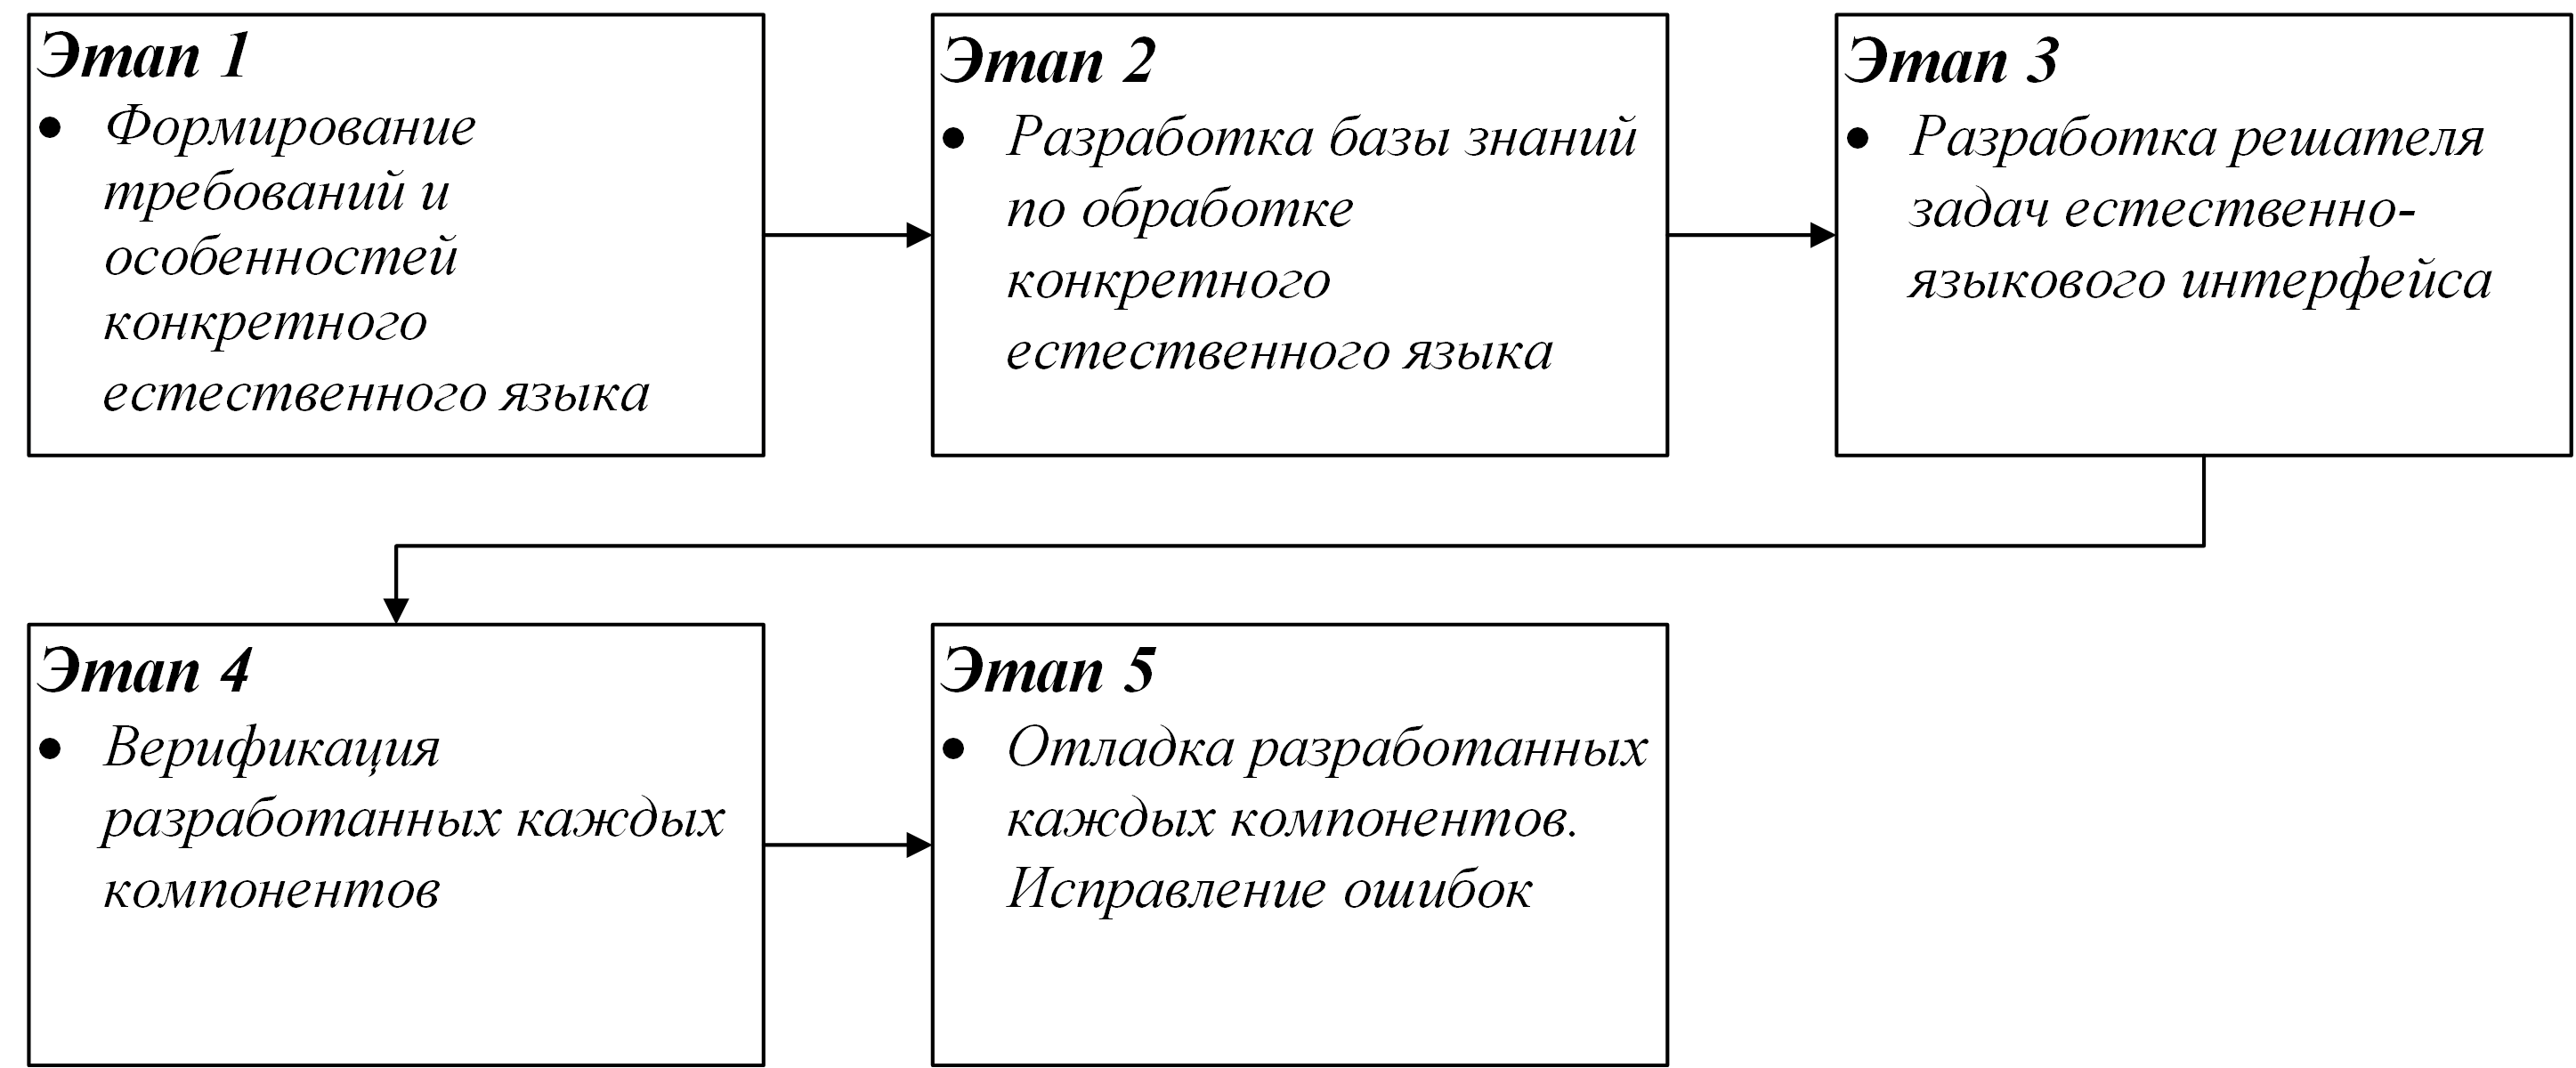
\includegraphics[scale=0.8,width=1.0\textwidth]{images/part4/chapter_chinese/method.png}
	\caption{Этапы процесса разработки естественно-языкового интерфейса}
	\label{fig:method-interface}
\end{figure}

Данная методика может быть применена при разработке конкретного естественно-языкового интерфейса по конкретной предметной области. Далее рассмотрим процесс разработки естественно-языкового интерфейса ostis-систем на этапах:

\textbf{Этап 1. Формирование требований и особенностей конкретного естественного языка.}

На данном этапе необходимо четко рассматривать особенности конкретного естественного языка. Затем можно разработать базу знаний по обработке конкретного естественного языка и соответствующие решатели задач для обработки конкретного естественного языка. После установления конкретного естественного языка существует вероятность того, что в составе библиотеки компонентов уже есть реализованный вариант требуемой базы знаний и соответствующих решателей. В противном случае, тем не менее, у разработчика появляется возможность включить разработанную базу знаний по обработке конкретного естественного языка и соответствующие решатели задач в библиотеку компонентов для последующего использования.

\textbf{Этап 2. Разработка базы знаний по обработке конкретного естественного языка.}

Общие принципы на основе методики согласованного построения и модификации гибридных баз знаний (см. \scncite{Davydenko2017}) используются для разработки базы знаний по обработке конкретного естественного языка.

\textbf{Этап 3. Разработка решателей задач естественно-языковых интерфейсов.}

Общие принципы на основе методики согласованного построения и модификации гибридных решателей задач (см. \scncite{Shunkevich2018}) используются для разработки решателей задач естественно-языкового интерфейса для решения задач приобретения фактографических знаний и генерации текстов конкретного естественного языка.

\textbf{Этап 4. Верификация разработанных каждых компонентов.}

На данном этапе верификация разработанных компонентов (база знаний по обработке конкретного естественного языка и соответствующие решатели задач для решения задач приобретения фактографических знаний и генерации текстов конкретного естественного языка) конкретного естественно-языкового интерфейса может осуществляться вручную

\textbf{Этап 5. Отладка разработанных каждых компонентов. Исправление ошибок.}

Как правило, этапы 4, 5 могут выполняться циклически до тех пор, пока разработанные компоненты не будут соответствовать предъявляемым требованиям.

Библиотека многократно используемых компонентов является важнейшим понятием в рамках технологии OSTIS. С помощью Библиотеки многократно используемых компонентов естественно-языковых интерфейсов могут выбрать компоненты по требованию или набору компонентов в одной из библиотек и включить их в разрабатываемой конкретной естественно-языковой интерфейс других ostis-систем, т.е. разработанные компоненты естественно-языковых интерфейсов могут быть повторно использован при разработке естественно-языковых интерфейсов в других ostis-системах. Аналогично, для разработки конкретных естественно-языковых интерфейсов в других ostis-системах Библиотеки многократно используемых компонентов конкретных естественно-языковых интерфейсов тоже могут использованы повторно для сокращения сроки и трудоемкости разработки конкретных естественно-языковых интерфейсов. Была разработана Библиотеки многократно используемых компонентов естественно-языковых интерфейсов и Библиотеки многократно используемых компонентов китайско-языкового интерфейса в качестве средства для разработки естественно-языковых интерфейсов.
\begin{SCn}
	\scnheader{Библиотека многократно используемых компонентов естественно-языковых интерфейсов}
	\begin{scnrelfromset}{разбиение}
		\scnitem{Библиотека многократно используемых компонентов базы знаний естественно-языковых интерфейсов}
		\begin{scnindent}
			\scnidtf{Библиотека многократно используемых компонентов базы знаний лигвистики}
			\scnidtf{Библиотека многократно используемых компонентов базы знаний по обработке естественного языка}
		\end{scnindent}
		\scnitem{Библиотека многократно используемых компонентов решателей задач естественно-языковых интерфейсов}
		\begin{scnindent}
			\scnidtf{Библиотека многократно используемых компонентов решателей задач для обработки естественного языка}
		\end{scnindent}
	\end{scnrelfromset}
\end{SCn}

\begin{SCn}
	\scnheader{Библиотека многократно используемых компонентов китайско-языкового интерфейса}
	\begin{scnrelfromset}{разбиение}
		\scnitem{Библиотека многократно используемых компонентов базы знаний китайско-языкового интерфейса}
		\begin{scnindent}
			\scnidtf{Библиотека многократно используемых компонентов базы знаний по обработке китайского языка}
		\end{scnindent}
		\scnitem{Библиотека многократно используемых компонентов решателей задач китайско-языкового интерфейса}
		\begin{scnindent}
			\scnidtf{Библиотека многократно используемых компонентов решателей задач для обработки китайского языка}
		\end{scnindent}
	\end{scnrelfromset}
\end{SCn}

На данный момент на основе модели базы знаний лингвистики были разработаны онтологии предметных областей в качестве компонентов, описывающих различные виды лингвистических знаний, которые могут использоваться для реализации конкретных естественно-языковых интерфейсов:
\begin{scnitemize}
	\item Предметная область слов;
	\item Предметная область словосочетаний;
	\item Предметная область предложений;
	\item Предметная область параграфов;
	\item и другие.
\end{scnitemize}

Различные виды лингвистических знаний для обработки китайского языка были специфицированы с использованием разработанных онтологий предметных областей в базе знаний по обработке китайского языка, которые могут быть разработаны в качестве компонентов для разработки китайско-языкового интерфейса в большинстве других ostis-систем.
\begin{scnitemize}
	\item Предметная область единиц сегментации;
	\item Предметная область словосочетаний китайского языка;
	\item Предметная область предложений китайского языка;
	\item Предметная область параграфов китайского языка;
	\item и другие.
\end{scnitemize}

На данный момент на основе модели решателей задач естественно-языковых интерфейсов основное внимание уделено многократно используемым sc-агентам, входящим в состав решателей задач естественно-языковых интерфейсов:
\begin{SCn}
	\scnheader{Библиотека многократно используемых атомарных абстрактных sc-агентов естественно-языковых интерфейсов}
	\begin{scnrelfromset}{разбиение}
		\scnitem{Библиотека sc-агентов формирования структур фактографических знаний}
		\scnitem{Библиотека sc-агентов установления конкретных sc-конструкций}
		\scnitem{Библиотека sc-агентов перевода sc-конструкций в соответствующие им message triple}
	\end{scnrelfromset}
\end{SCn}

Аналогично, при разработке китайско-языкового интерфейса новой ostis-системы, многократно используемый абстрактный sc-агент нужно быть скопирован в этой новой ostis-системе, после того необходимо сгенерировать sc-узел, обозначающий конкретный sc-агент, работающий в этому китайско-языковом интерфейсе данной системы. На данный момент многократно используемым sc-агентам, входящим в состав решателей задач китайско-языкового интерфейса:
\begin{SCn}
	\scnheader{Библиотека многократно используемых атомарных абстрактных sc-агентов китайско-языкового интерфейса}
	\scnidtf{Библиотека многократно используемых атомарных абстрактных sc-агентов для обработки китайского языка}
	\begin{scnrelfromset}{разбиение}
		\scnitem{Библиотека sc-агентов разбиения текстов на единицы сегментации}
		\scnitem{Библиотека sc-агентов разметки отдельных единиц сегментации}
		\scnitem{Библиотека sc-агентов перевода конкретных sc-конструкций в соответствующие им message triple на китайском языке}
		\scnitem{Библиотека sc-агентов генерации текстов китайского языка из message triple}
	\end{scnrelfromset}
\end{SCn}

\subsection {Реализация китайско-языкового интерфейса}
На основе sc-модели естественно-языковых интерфейсов ostis-систем могут быть реализованы конкретные естественно-языковые интерфейсы интеллектуальных справочных систем по различным предметным областям. Однако из-за трудоемкости и сложности разработки интеллектуальных справочных систем по конкретным предметным областям, а также автор как носитель китайского языка, прототип китайско-языкового интерфейса был реализован в интеллектуальной справочной системе по дискретной математике.

\subsubsection{Извлечение фактографических знаний из текстов китайского языка}
Преобразование текстов естественного языка в фрагменты базы знаний рассматривается как задачи извлечения фактографических знаний. В данном случае преобразование текстов китайского языка в фрагменты базы знаний интеллектуальной справочной системы по дискретной математике заключается в извлечении именованных сущностей и отношений между ними из текстов китайского языка по дискретной математике, а наконец извлеченные результаты сохраняются в виде SC-кода в базе знаний интеллектуальной справочной системы по дискретной математике.

Несколько требований былы определены для задач преобразования текстов китайского языка в фрагменты базы знаний:
\begin{textitemize}
	\item Вход представляет собой стандартное повествовательное предложение китайского языка, а не речевое;
	\item Входное повествовательное предложение китайского языка имеет завершенный смысл и фактографическое знание;
	\item Не нужен заранее заданный словарь, включающий заранее определенные типы именованных сущностей и отношений между ними;
	\item Выход представляет собой sc-структура, формально представленная в базе знаний.
\end{textitemize}

В данном подразделе показан пример процесса анализа предложения китайского языка, которое представлено на таком узле на рисунке \textit{\nameref{fig:chinese-sentence-sc}}. Содержимое такого узла демонстрирует предложение китайского языка, которое относится к области дискретной математики и описывает: \begin{CJK}{UTF8}{gbsn}«从结构形式化的角度 (с точки зрения формализации структуры) ,结构(структуру) 可以 (можно) 划分 (разделить) 为 (на) 形式化的结构 (формальную структуру) 和 (и) 非形式化的结构 (неформальную структуру) 。». \end{CJK}
\begin{figure}[H]
	\centering
	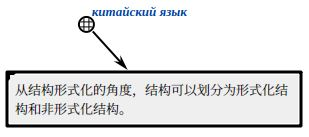
\includegraphics[scale=0.8]{images/part4/chapter_chinese/chinese_sentence.png}
	\caption{Представление предложения китайского языка в ostis-системе}
	\label{fig:chinese-sentence-sc}
\end{figure}

\textbf{\textit{Шаг 1:}} Декомпозиция предложения китайского языка на отдельные единицы сегментаций, а также помечаются данные единицы сегментаций стандартными категориями частей речи в китайском языке (рисунок \textit{\nameref{fig:segment-chinese}}).
\begin{figure}[H]
	\centering
	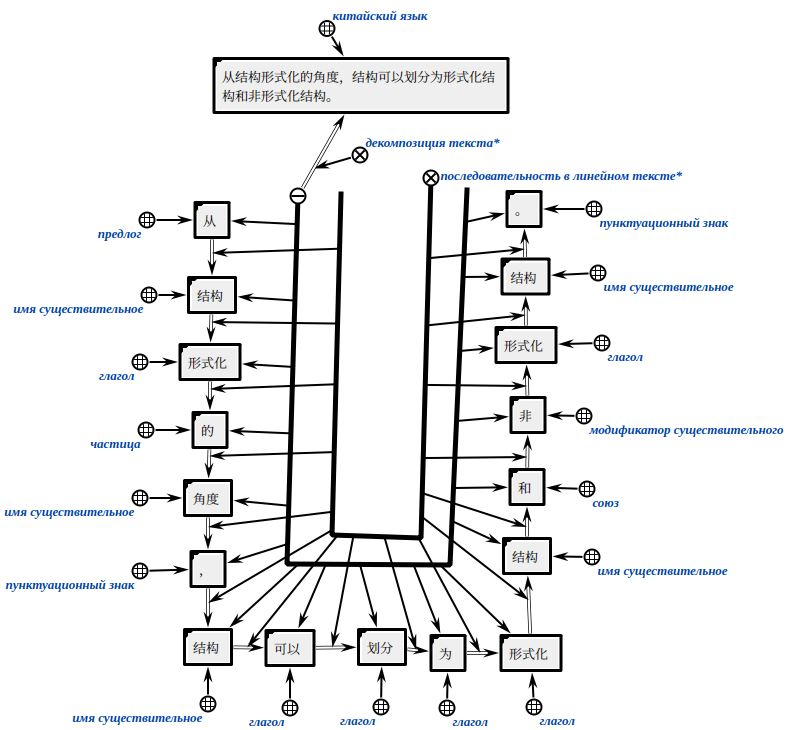
\includegraphics[scale=0.6]{images/part4/chapter_chinese/segment_chinese_sentence.png}
	\caption{Результат разделения и разметки отдельных единиц сегментации}
	\label{fig:segment-chinese}
\end{figure}

Согласно особенности текстов китайского языка, текст китайского языка состоит из потока иероглифов без естественных пробелов на основе письменной формы. При этом в китайском языке отсутствуют четкие показатели категорий числа, падежа и рода, такие как в русском языке и других европейских языках, функция слова в китайском языке становится понятной не на основании морфологических изменений слова, а благодаря его связи с другими словами. В связи с этим в процессе анализа текстов китайского языка сначала необходимо выполнить лексический анализ, разбивающий поток иероглифов в тексте китайского языка на отдельные значимые единицы сегментации китайского языка. 

\textbf{\textit{Шаг 2:}} Синтаксический анализ выполняет построение синтаксической структуры предложения китайского языка (рисунок \textit{\nameref{fig:syntac-structure}}).

При обработке китайского языка синтаксический анализ являются анализом взаимосвязей (или отношений зависимости) между входными предложениями китайского языка и раздельными единицами сегментаций и между раздельными единицами сегментации в предложениях китайского языка для раскрытия их синтаксических структур. На основе построенной синтаксической структуры приложений китайского языка фактографические знания можно быть извлечены с использованием правил извлечения. Таким образом, синтаксический анализ китайского языка позволяет создать основу для извлечения фактографических знаний из предложений китайского языка.
\begin{figure}[H]
	\centering
	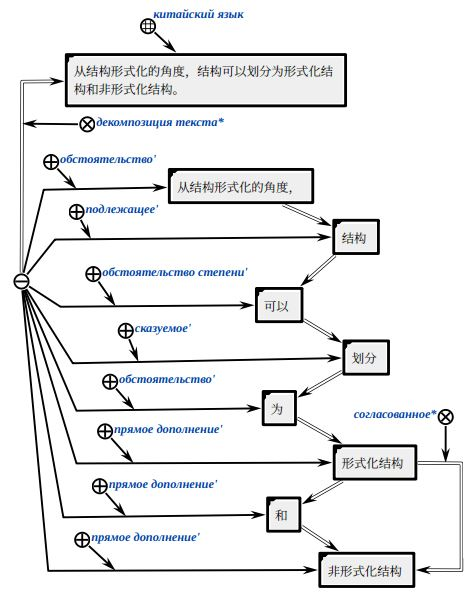
\includegraphics[scale=0.6]{images/part4/chapter_chinese/syntac_structure.png}
	\caption{Результат синтаксического анализа предложения китайского языка}
	\label{fig:syntac-structure}
\end{figure}

При обработке китайского языка отношения между единицами сегментации и входным предложением китайского языка, или отношения между единицами сегментации в предложения китайского языка, обычно рассматриваются как определенные типы лингвистических знаний, включенных в базе знаний по обработке китайского языка.

\textbf{\textit{Шаг 3:}} На основе результата синтаксического анализа входного предложения китайского языка фактографические знания (именованные сущности и отношения между ними) извлекаются из предложения с использованием правил извлечения, т.е. построение фрагмента базы знаний в базе знаний интеллектуальной справочной системы.


\begin{figure}[H]
	\centering
	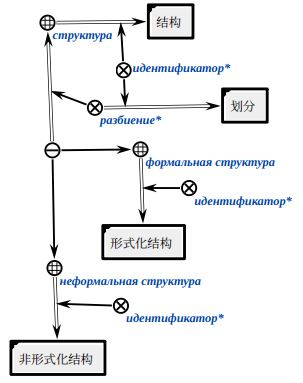
\includegraphics[scale=0.7]{images/part4/chapter_chinese/generated_sc_structure.png}
	\caption{Результирующий построенный фрагмент в базе знаний}
	\label{fig:generated-structure}
\end{figure}

С точки зрения извлечения фактографических знаний из открытой области, основными задачами является извлечение именованных сущностей и отношений между ними из предложений китайского языка, не требуя предопределенных типов именованных сущностей и отношений. Фактически, в рамках \scnkeyword{Технологии OSTIS} отношение рассматривается как специальная сущность, которая определяет определенное отношение между парами независимых именованных сущностей, которое обычно представлена соответственно как sc-узел, обозначающий ролевое отношение в форме SCg-кода.

В целом, пары независимых именных сущностей должны появляться в анализируемой синтаксической структуре в виде именных фраз, относящихся к номинативным единицам. В дальнейшем связи между этими именными фразами и входным предложением китайского языка, а также путь, связывающий две именные фразы через другие единицы сегментаций, будут отражать соответствующие отношения между парами именных сущностей. Более точно, именные фразы, появляющиеся в анализируемой синтаксической структуре входного предложения китайского языка, представляются как идентификаторы sc-узлов, обозначающих название некоторых именованных сущностей, хранящихся в базе знаний интеллектуальной справочной системы по дискретной математике.

На рисунке \textit{\nameref{fig:generated-structure}} показан построенный фрагмент базы знаний из входного предложения китайского языка в базе знаний интеллектуальной справочной системы по дискретной математике без обнаружения противоречий. В данном случае фрагмент базы знаний может быть построен напрямую без связывания именованных сущностей, упомянутых во входном исходном предложении китайского языка, с соответствующими существующими определенными именованными сущностями в базе знаний интеллектуальной справочной системы по дискретной математике. В некоторых случаях для именованной сущности в базе знаний существуют различные названия в текстах естественного языка для описания этой именованной сущности. В этом случае необходимо выполнить устранение противоречий, чтобы связать разные именованные сущности (именно идентификаторы именованных сущностей) в текстах естественного языка с одинаковыми именованными сущностями в базе знаний ostis-системы. 
\subsubsection{Генерация текстов из фрагментов базы знаний}
Для реализации генерации текстов китайского языка из фрагментов базы знаний ostis-системы условно делится на два этапа: символьные генераторы, преобразующие фрагменты (sc-структуры) базы знаний в соответствующие им ``message triple''; генераторы на основе шаблонов или статистические генераторы (при наличии высококачественных выровненных наборов данных), переводящие ``message triple'' в результирующие тексты китайского языка. Пример генерации текстов китайского языка демонстрирует процесс генерации повествовательного предложения китайского языка на основе правил и шаблонов.

Из-за сложности и разнообразия задач генерации текстов, при генерации текстов китайского языка из фрагментов базы знаний ostis-системы соблюдаются следующие ограничения:
\begin{textitemize}
	\item входной фрагмент базы знаний обладает законченной sc-структурой и конкретным смыслом;
	\item выходным результатом является повествовательное предложение китайского языка;
	\item входной фрагмент базы знаний содержит sc-элементы (представляющие сущности, отношения, класс сущностей или другие) с идентификаторами на китайском языке, которые будут использоваться в результирующих предложениях китайского языка.
\end{textitemize}

\textbf{\textit{Шаг 1:}} Локализация заданного фрагмента (sc-структура) из базы знаний интеллектуальной справочной системы по дискретной математике, представленного в виде SC-кода и содержащего sc-элементы с идентификаторами на китайском языке. Для визуального представления данного фрагмента базы знаний, фрагмент формально представлен в виде SCg (рисунок \textit{\nameref{fig:knowledge-base-fragment}}).
\begin{figure}[H]
	\centering
	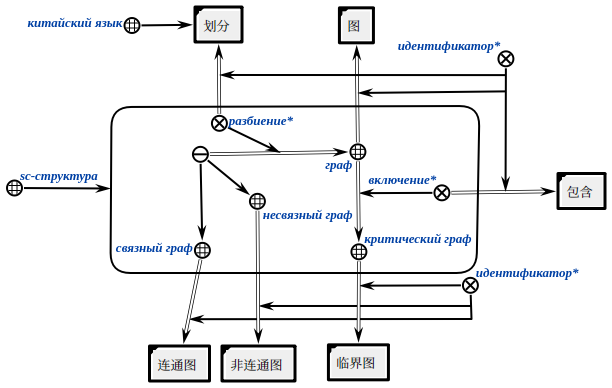
\includegraphics[scale=0.7]{images/part4/chapter_chinese/fragment_knowledge_base.png}
	\caption{Фрагмент (sc-структура) базы знаний ИСС по дискретной математике}
	\label{fig:knowledge-base-fragment}
\end{figure}

\textbf{\textit{Шаг 2:}} Данный фрагмент разделяется на стандартные базовые sc-конструкции, из которых выбираются проектные sc-конструкции для генерации результирующих текстов китайского языка, которые можно переводиться в ``message triple''. У каждого sc-элемента sc-конструкций есть конкретная единица сегментации китайского языка, соответствующая идентификатору каждого sc-элемента. Проектная sc-конструкция (принадлежащая к стандартной базовой sc-конструкции) показана на SCg (рисунок \textit{\nameref{fig:candidate-sc-construction}}).
\begin{figure}[H]
	\centering
	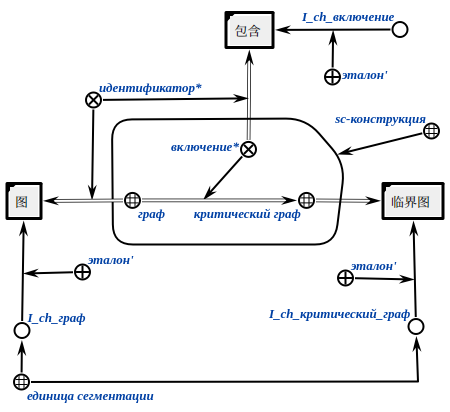
\includegraphics[scale=0.8]{images/part4/chapter_chinese/candidate_sc_structure.png}
	\caption{Выбранная проектная sc-конструкция}
	\label{fig:candidate-sc-construction}
\end{figure}

\textbf{\textit{Шаг 3:}} Проектная sc-конструкция переносится в ``message triple''. Преобразованный ``message triple'' состоит из файлов (sc-узел с содержимым), содержащих единицы сегментаций, написанные обученными носителями китайского языка и проверенной другими. Содержимое некоторых файлов (например \begin{CJK}{UTF8}{gbsn} «临界图 (критический граф)» \end{CJK}) соответствует идентификатору sc-элементов sc-конструкций, а содержимое некоторых файлов добавляется при построении ``message triple''. (рисунок \textit{\nameref{fig:message-triple}}).
\begin{figure}[H]
	\centering
	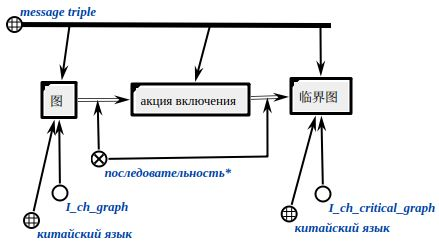
\includegraphics[scale=0.7]{images/part4/chapter_chinese/message_triple.png}
	\caption{Перевод проектной sc-конструкции в ``message triple''}
	\label{fig:message-triple}
\end{figure}

\textbf{\textit{Шаг 4:}} файлы объединяются для генерации результирующего повествовательного предложения китайского языка в соответствии с допустимыми упорядоченностями на шаблоне для ``message triple'' с отношением «включение» (рисунок \textit{\nameref{fig:sentence-generated}}). При генерации результирующих текстов для некоторых естественных языков Формы слов изменяются в соответствии с правилами (например, заглавная буква первого слова в предложении, согласование сказуемого с подлежащим), а затем добавляются в результирующие тексты. \textit{Ссылающееся выражение*} -- квазибинарное отношение, связывающее слово с её комбинаторными вариантами. 
\begin{figure}[H]
	\centering
	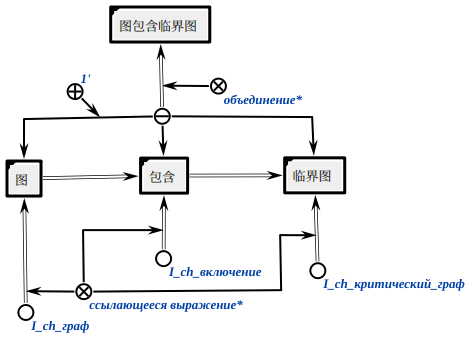
\includegraphics[scale=0.7]{images/part4/chapter_chinese/chinese_sentence_generated.png}
	\caption{Генерация предложения китайского языка, соответствующего sc-структуре}
	\label{fig:sentence-generated}
\end{figure}

В отличие от европейских языков, склоняемая форма лексических единиц (например, единственного или множественного числа и других форм склонения) в файлах указывается в результирующих текстах в соответствии с синтаксическими правилами конкретного естественного языка. Однако в связи с особенностями китайского языка, обработка данного шага относительно проще. В данном примере при генерации результирующего предложения китайского языка, ссылочное выражение каждой единицы сегментации означает конечную форму единицы сегментации в результирующем предложении китайского языка. Исходя из шаблона, в качестве подлежащего выступает ссылочное выражение к единице сегментации \begin{CJK}{UTF8}{gbsn} «图 (граф)» \end{CJK}. Единица сегментации \begin{CJK}{UTF8}{gbsn} «临界图 (критический граф)» \end{CJK} выступает в качестве объекта. Сгенерированное предложение китайского языка описывает \begin{CJK}{UTF8}{gbsn}«图 (граф) 包含 (включение) 临界图 (критический граф)». \end{CJK}

Некоторые отношения уже предопределены в \scnkeyword{IMS} (см. \scncite{IMS}) системе для разработки ostis-системы, так \textit{включение*}, \textit{эквиваленция*} и так далее. Для данных конечных отношений, предопределенных в \scnkeyword{IMS} системе, будем называть доменно-независимые отношения. Для бесконечных доменно-зависимых отношений в различных предметных областей модель нейронной сети интегрирована в решатель задач к генерации текстов китайского языка. На рисунке \textit{\nameref{fig:pre-training-model}} показан процесс использовании формы предварительной подготовки и тонкой настройки для решения задач генерации текстов китайского языка из фрагментов базы знаний. 
\begin{figure}[H]
	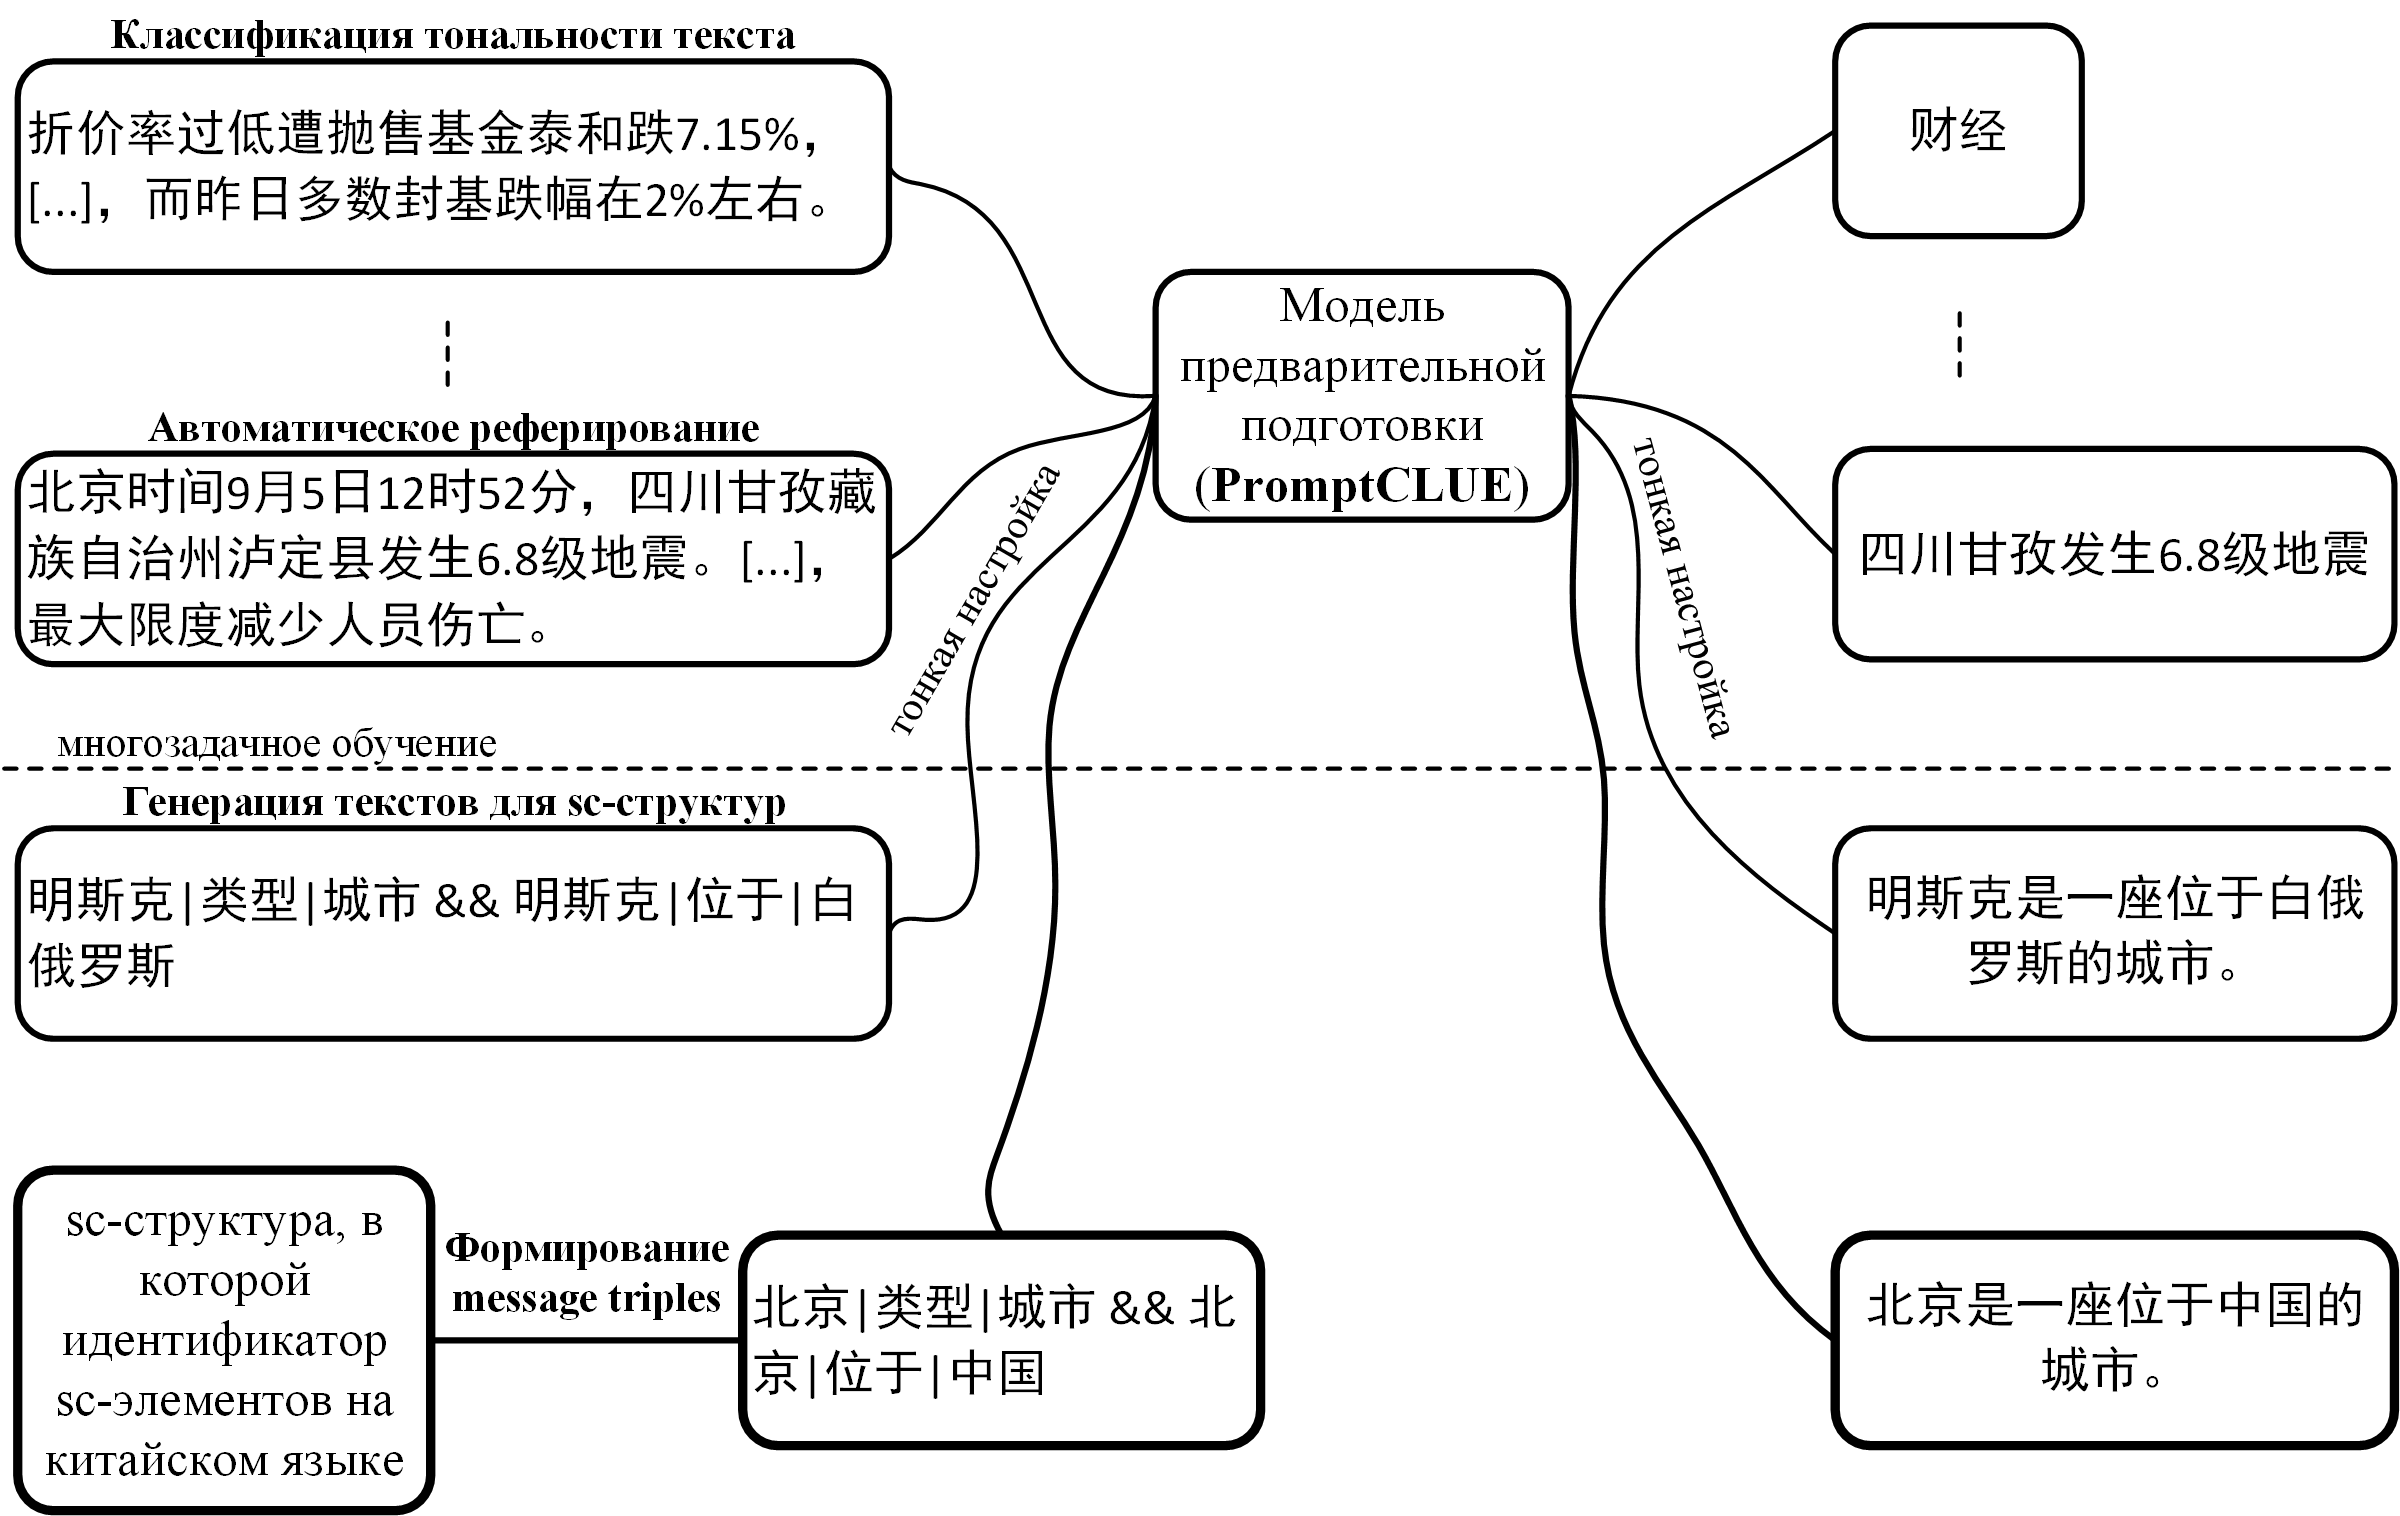
\includegraphics[scale=0.8,width=1.0\textwidth]{images/part4/chapter_chinese/promptCLUE4SC.png}
	\caption{Диаграмма для генерации текстов на основе модели предварительной подготовки PromptCLUE}
	\label{fig:pre-training-model}
\end{figure}

Как видно из рисунка \textit{\nameref{fig:pre-training-model}}, была использована модель предварительной подготовки PromptCLUE, которая использует еncoder-decoder архитектуру на основе модели Transformer и предварительно обучается на нескольких наборов задач про обработке китайского языка (классификация тональности текста, автоматическое реферирование и другие) с использованием огромного китайского корпуса (сотни ГБ китайского корпуса).  На основе модели PromptCLUE, проведена тонкая настройка с использованием построенных корпусов для генерации текстов китайского языка из фрагментов базы знаний (sc-структур) в виде пары ``message triple''/предложение китайского языка. После обучения тонкой настройки на модели PromptCLUE, обученная модель может быть использована для генерации текстов китайского языка после предварительной обработки sc-структур в ``message triple''. 

\section*{Заключение}
В главе предложена на основе \scnkeyword{Технологии OSTIS} единая семантическая модель естественно-языковых интерфейсов интеллектуальных систем для разработки естественно-языковых интерфейсов, которые имеют возможность преобразовывать тексты естественного языка в фрагменты базы знаний и генерировать тексты естественного языка из фрагментов базы знаний интеллектуальных систем. Разработка семантической модели естественно-языковых интерфейсов в основном включает разработка SC-модели базы знаний лингвистики, которая представлена в виде описанных предметных областей и соответствующих им онтологий по лингвистическим знаниям для обработки естественного языка, а также SC-модели решателей задач естественно-языковых интерфейсов, разработанной как иерархическая система sc-агентов, которая позволяет интегрировать различные модели решения задач (например логические модели на основе правил, модели нейронных сетей и другие) для обработки естественного языка.

С помощью предложенной семантической модели естественно-языковых интерфейсов реализован прототип китайско–языкового интерфейса ИСС по дискретной математике, способный решать задачи преобразования текстов китайского языка в фрагменты базы знаний и генерации текстов китайского языка из фрагментов базы знаний. Для реализации китайско–языкового интерфейса разработана база знаний по обработке китайского языка и соответствующие решатели задач анализа текстов и генерации текстов китайского языка.
%\input{author/references}